\documentclass{myclass}
\usepackage[polish]{babel}

\setcounter{secnumdepth}{3}
\author{Bartosz Hanc}
% Based on 
%   ,,Wstęp do mechaniki kwantowej'', D.J. Griffiths, D.V. Schroeder;

%   ,,Teoria kwantów. Mechanika falowa.'', I. Białynicki--Birula, M. Cieplak, J. Kamiński;

%   ,,Krótki kurs fizyki teoretycznej. Tom 2.'', L.D. Landau, J. Lifszyc.


\begin{document}

\newgeometry{total={6in, 9in}}
\onecolumn
\tableofcontents

\newpage

\restoregeometry

\section*{Podstawy mechaniki kwantowej}

\textit{It seems clear that the present quantum mechanics is not in its final form
\ldots}\begin{flushright}P.A.M. Dirac\end{flushright}

\subsection{Wprowadzenie}

\subsubsection{Równanie Schr{\"o}dingera}

Rozpatrzmy następujący problem: cząstka o masie \(m\) znajduje się w polu potencjalnym o potencjale
\(V(\mathbf{r},t)\). Chcemy znaleźć jej trajektorię \(\mathbf{r}(t)\) dla ustalonych warunków
początkowych \(\mathbf{r}(0)\), \(\dot{\mathbf{r}}(0)\). W nierelatywistycznej mechanice klasycznej
należałoby więc rozwiązać równanie różniczkowe

\begin{equation*}
    \ddot{\mathbf{r}}=-\frac{1}{m}\nabla V(\mathbf{r},t)\,.
\end{equation*}
Doświadczenia jednakże dobitnie pokazują, iż takie klasyczne podejście jest zupełnie nieadekwatne
dla obiektów z mikroświata. Poprawnym równaniem opisującym takie cząstki jest \underline{równanie
Schr{\"o}dingera}

\begin{equation*}
    \boxed{\left[-\frac{\hbar^2}{2m}\Delta+V(\mathbf{r},t)\right]\Psi=\im\hbar\pdv{\Psi}{t}}
\end{equation*}
gdzie \(\hbar\) jest zredukowaną stałą Plancka. Funkcję
\(\Psi(\mathbf{r},t):\mathbb{R}^4\mapsto\mathbb{C}\) nazywamy \underline{funkcją falową} cząstki.
\subsubsection{Interpretacja Borna funkcji falowej}
Czym właściwie fizycznie jest \(\Psi(\mathbf{r},t)\)? W interpretacji statystycznej Borna mówimy, iż
znaczenie fizyczne ma jedynie rzeczywista wielkość \(\Psi^*\Psi=|\Psi|^2\), która określa
\underline{gęstość prawdopodobieństwa} znalezienia w chwili \(t\) cząstki w punkcie \(\mathbf{r}\),
tj. wielkość

\begin{equation*}
    P_D(t)=\iiint_D\Psi^*\Psi\dd{^3\mathbf{r}}
\end{equation*}
jest prawdopodobieństwem znalezienia cząstki w obszarze \(D\) w ustalonej chwili \(t\).

\subsubsection{Problem pomiaru i kolaps funkcji falowej}

Teoria kwantowa pozwala stwierdzić jedynie, z jakim prawdopodobieństwem możemy znaleźć cząstkę w
pewnym otoczeniu punktu \(\mathbf{r}\). Dokonując pomiaru jej położenia, stwierdzamy jednakże, iż
cząstka ma konkretne położenie \(\mathbf{r}_\text{o}\) (oczywiście w granicach niepewności
pomiarowych przyrządów). Co więcej, natychmiastowe powtórzenie pomiaru położenia nie zmienia wyniku
tj. cząstka nadal jest w punkcie \(\mathbf{r}_\text{o}\) tak długo, jak ją tam mierzymy. Zjawisko to
nazywamy \underline{kolapsem funkcji falowej}. W takim razie akt pomiaru drastycznie zmienia funkcję
falową.
\medskip

\textit{Te obserwacje były i nadal są punktem wyjścia dla poważnych rozważań filozoficznych. My
przyjmiemy jednak \underline{postawę aksjomatyczną} usprawiedliwioną mnogością zastosowań teorii
opartej na tych nieintuicyjnych postulatach.}

\subsubsection{Postulaty}

Założymy więc, iż
\begin{itemize}

    \item Stan cząstki kwantowej o masie \(m\) jest opisywany funkcją
    \(\Psi(\mathbf{r},t):\mathbb{R}^4\mapsto\mathbb{C}\), którą nazywamy \underline{funkcją falową}.

    \item Interpretację fizyczną nadajemy jedynie rzeczywistej wielkości \(\Psi^*\Psi\), którą
    interpretujmy jako \underline{gęstość prawdopodobieństwa} znalezienia cząstki w położeniu
    \(\mathbf{r}\) w danej chwili \(t\), tj.
    
    \begin{equation*}
        P_D(t)=\iiint_D\Psi^*\Psi\dd{^3\mathbf{r}}
    \end{equation*}
    jest prawdopodobieństwem znalezienia cząstki w obszarze \(D\) w chwili \(t\).

    \item Przy braku ,,zewnętrznej ingerencji'' w układ funkcja \(\Psi\) spełnia równanie
    Schr{\"o}dingera

    \begin{equation*}
        \left[-\frac{\hbar^2}{2m}\Delta+V(\mathbf{r},t)\right]\Psi=\im\hbar\pdv{\Psi}{t}\,.
    \end{equation*}

    \item Ingerencja w układ powoduje kolaps funkcji falowej, który utrzymuje się tak długo, jak
    długo obecna jest ,,zewnętrzna ingerencja'' i objawia się nieciągłą zmianą gęstości
    prawdopodobieństwa do postaci funkcji delta Diraca

    \begin{equation*}
        |\Psi(\mathbf{r},t)|^2=\delta^3(\mathbf{r}-\mathbf{r}_\text{o})
    \end{equation*}
    gdzie \(\mathbf{r}_\text{o}\) jest \underline{zmierzonym} położeniem cząstki.

    \item Po zaprzestaniu ingerencji funkcja falowa znów ewoluuje zgodnie z równaniem
    Schr{\"o}dingera, przy czym warunki brzegowe są dane przez jej postać w stanie kolapsu.

    \item \hyperref[postulat1]{Postulat o wartości oczekiwanej} [\textit{wyjaśnienie dalej}]

    \item \hyperref[postulat2]{Postulat o uogólnionej interpretacji statystycznej}
    [\textit{wyjaśnienie dalej}]

\end{itemize}

\subsubsection{Normalizacja}

Przyjmując interpretację statystyczną, musimy mieć pewność, iż funkcja falowa jest
\underline{unormowana} dla wszystkich chwil \(t\), tj. dla każdego \(t\) zachodzi

\begin{equation*}
    \iiint_{\mathbb{R}^3}\Psi^*\Psi\dd{^3\mathbf{r}}=1\,.
\end{equation*}
Zauważmy, iż jeśli \(\Psi\) spełnia równanie Schr{\"o}dingera to \(\Psi'=\alpha\Psi\) dla pewnej
liczby zespolonej \(\alpha\) również je spełnia. W takim razie szukamy stałej
\(\alpha\in\mathbb{C}\) takiej, że dla danego rozwiązania równania Schr{\"o}dingera \(\Psi\) funkcja
\(\alpha\Psi\) spełniała \underline{warunek unormowania}. Jeśli dla danej \(\Psi\) nie jest to
możliwe to taką funkcję falową nazywamy \underline{nienormowalną} i odrzucamy jako niezgodną z
interpretacją Borna. Jednocześnie powyższa całka nie może być zależna od chwili \(t\), w której ją
obliczamy. Na szczęście można udowodnić, iż tak właśnie jest. Istotnie

\begin{equation*}
    \dv[]{}{t}\iiint_{\mathbb{R}^3}\Psi^*\Psi\dd{^3\mathbf{r}}=\iiint_{\mathbb{R}^3}\left(\Psi\pdv{\Psi^*}{t}+\Psi^*\pdv{\Psi}{t}\right)\dd{^3\mathbf{r}}\,.
\end{equation*}
Jeśli \(\Psi\) spełnia równanie Schr{\"o}dingera

\begin{equation*}
    \left[-\frac{\hbar^2}{2m}\Delta+V(\mathbf{r})\right]\Psi=\im\hbar\pdv{\Psi}{t}
\end{equation*}
to biorąc sprzężenie zespolone obu stron równości otrzymujemy

\begin{equation*}
    \im\hbar\pdv{\Psi^*}{t}=\left[+\frac{\hbar^2}{2m}\Delta -V\right]\Psi^*\,,
\end{equation*}
przy czym założyliśmy tutaj, iż \(\boxed{V\in\mathbb{R}}\). W takim razie

\begin{equation*}
    \Psi\pdv{\Psi^*}{t}+\Psi^*\pdv{\Psi}{t}=\frac{\im\hbar}{2m}\left(\Psi^*\Delta\Psi-\Psi\Delta\Psi^*\right)\,.
\end{equation*}
Korzystając z drugiej tożsamości Greena mamy więc

\begin{equation*}
    \iiint_{\mathbb{R}^3}\pdv{(\Psi^*\Psi)}{t}\dd{^3\mathbf{r}}=\frac{\im\hbar}{2m}\oiint_{\partial\mathbb{R}^3}(\Psi^*\nabla\Psi-\Psi\nabla\Psi^*)\cdot\dd{\mathbf{S}}
\end{equation*}
ale ze względu na fakt, iż przy \(|\mathbf{r}|\to\infty\) funkcja falowa musi dążyć do 0 (aby była
normowalna) całka po prawej jest po prostu równa 0 \(\blacksquare\)
\medskip

Zauważmy jeszcze, iż w przypadku ograniczonego obszaru \(D\subset \mathbb{R}^3\) mamy z powyższego

\begin{equation*}
\dv[]{P_D}{t}=-\frac{\hbar}{2m\im}\oiint_{\partial D}(\Psi^*\nabla\Psi-\Psi\nabla\Psi^*)\cdot\dd{\mathbf{S}}\,,
\end{equation*}
czyli interpretując wielkość \(\mathbf{J}:=\frac{\hbar}{2m\im}(\Psi^*\nabla\Psi-\Psi\nabla\Psi^*)\)
jako \underline{gęstość prądu prawdopodobieństwa}, widzimy, iż spełnione jest równanie ciągłości

\begin{equation*}
\nabla\cdot\mathbf{J}=-\pdv{\rho}{t}\,,
\end{equation*}
gdzie oczywiście \(\rho=\Psi^*\Psi\).
\medskip

\noindent\rule{\columnwidth}{0.5pt}\\
\textcolor{purple}{Jeśli \(V\in\mathbb{C}\) i oznaczymy \(V=\alpha+\im\beta\) to z faktu, iż
\(\Psi\) spełnia równanie Schr{\"o}dingera mamy
\begin{equation*}
-\frac{\hbar^2}{2m}\Delta\Psi^*+(\alpha-\im\beta)\Psi^*=-\im\hbar\pdv{\Psi^*}{t}\,,
\end{equation*}
skąd
\begin{equation*}
    \Psi\pdv{\Psi^*}{t}+\Psi^*\pdv{\Psi}{t}=\frac{\im\hbar}{2m}(\Psi^*\Delta\Psi-\Psi\Delta\Psi^*)+\frac{2\beta}{\hbar}\Psi^*\Psi\,.
\end{equation*}
W takim razie otrzymujemy
\begin{equation*}
    \dv[]{P}{t}=\iiint_{\mathbb{R}^3}\pdv{(\Psi^*\Psi)}{t}\dd{^3\mathbf{r}}=\frac{2\beta}{\hbar}\iiint_{\mathbb{R}^3}\Psi^*\Psi\dd{^3\mathbf{r}}\,.
\end{equation*}
W takim przypadku prawdopodobieństwo \(P\) znalezienia cząstki gdziekolwiek w przestrzeni nie jest
stale równe 1, tylko maleje (dla \(\beta<0\)) zgodnie ze wzorem
\begin{equation*}
    P(t)=\exp{\frac{2\beta}{\hbar}t}\,.
\end{equation*}
W takim przypadku opisujemy niestabilną cząstkę, która rozpada się po upływie jej czasu życia
\(\tau=-\frac{1}{2}\hbar\beta^{-1}\).}\\
\noindent\rule{\columnwidth}{0.5pt}

\subsubsection{Operatory i wartość oczekiwana}

\begin{itemize}

    \item \underline{Wartość oczekiwaną} (wartość średnią) funkcji \(f(x)\) przy jednowymiarowym
    rozkładzie prawdopodobieństwa danym funkcją gęstości \(\rho(x)\) definiujemy jako
    \begin{equation*}
        \langle f\rangle := \int\limits_{-\infty}^{+\infty}f(x)\rho(x)\dd{x}\,.
    \end{equation*}

    \item \underline{Odchylenie standardowe \(\sigma\)} funkcji \(f(x)\) dla rozkładu
    prawdopodobieństwa danego funkcją gęstości \(\rho(x)\) definiujemy jako
    \begin{equation*}
        \sigma_f:=\sqrt{\langle f^2\rangle-\langle f\rangle^2}=\sqrt{\left\langle(f-\langle f\rangle)^2\right\rangle}\,.
    \end{equation*}
    Wielkość \(\sigma^2\) nazywamy \underline{wariancją}.
    \end{itemize}
\label{postulat1}W mechanice kwantowej interpretację statystyczną rozszerzamy dodatkowo o
\underline{postulat} (który nazwiemy ,,postulatem o wartości oczekiwanej''), iż wartość oczekiwaną
mierzalnej podstawowej wielkości dynamicznej (np. \(x\), \(p_x\), \(H\)) zależnej od położenia i
pędu \(Q(x,p)\) obliczamy jako

\begin{equation*}
            \boxed{\langle Q \rangle=\iiint_{\mathbb{R}^3}\Psi^*\left[\hat{Q}\left(x,-\im\hbar\pdv{ }{x}\right)\right]\Psi \dd{^3\mathbf{r}} }\,,
\end{equation*}
gdzie \(\hat{Q}\) jest \underline{operatorem kwantowo-mechanicznym} powstałym z wielkości
dynamicznej \(Q\) przez podstawienie \(p_x\mapsto-\im\hbar\pdv{ }{x}\) (analogicznie dla \(p_y\),
\(p_z\)) i \(x\mapsto x\) (analogicznie dla \(y\), \(z\)). Operator \(\hat{p}\) nazywamy
\underline{operatorem pędu}, natomiast operator \(\hat{x}\) -- \underline{operatorem położenia}.
Wartość oczekiwana \(\langle Q\rangle\) określa średnią z pomiarów wielkości dynamicznej \(Q\) na
wielu \underline{oddzielnych} cząstkach (układach) opisywanych zadaną funkcją falową \(\Psi\)
(mówimy o cząstkach znajdujących się w stanie \(\Psi\)).\\

\textbf{Uwaga!} Przy definiowaniu operatora oprócz podania wyniku jego działania na funkcję falową
\(\Psi\) należy podać jego \underline{dziedzinę} tj. zbiór funkcji falowych (np.
\(L^2_\mathbb{C}[\mathbb{R}]\)) na które działa.
\medskip

Mówimy, iż pewne dwa operatory \(\hat{A}\) i \(\hat{B}\) \underline{komutują} wtedy i tylko wtedy,
gdy zachodzi

\begin{equation*}
    \hat{A}(\hat{B}\Psi)=\hat{B}(\hat{A}\Psi)\,.
\end{equation*}

\underline{Komutatorem} operatorów \(\hat{A}\) i \(\hat{B}\) nazywamy operator \([\hat{A},\hat{B}]\)
zdefiniowany jako

\begin{equation*}
    [\hat{A},\hat{B}]:=\hat{A}(\hat{B}(\cdot))-\hat{B}(\hat{A}(\cdot))\,.
\end{equation*}

Łatwo pokazać, iż \(\left[x,-\im\hbar\pdv{ }{x}\right]=\im\hbar\). Zależność tę nazywamy
\underline{kanoniczną relacją komutacyjną}.\\
Dla dowolnych operatorów \(\hat{A}\), \(\hat{B}\), \(\hat{C}\) zachodzi

\begin{equation*}
    \begin{split}
        &[\hat{A}+\hat{B},\hat{C}]=[\hat{A},\hat{C}]+[\hat{B},\hat{C}]\\
        &[\hat{A}\hat{B},\hat{C}]=\hat{A}[\hat{B},\hat{C}]+[\hat{A},\hat{C}]\hat{B}
    \end{split}
\end{equation*}

\subsection{Formalizm}

Podstawowymi wielkościami w mechanice kwantowej są funkcje falowe \(\Psi\), które
\underline{reprezentują stan układu} oraz operatory \(\hat{Q}\), które \underline{reprezentują tzw.
obserwable}, czyli mierzalne, podstawowe wielkości dynamiczne. Ze względu na warunek normalizacji

\begin{equation*}
\iiint_{\mathbb{R}^3}\Psi^*\Psi\dd{^3\mathbf{r}}=1<+\infty
\end{equation*}
funkcje falowe reprezentujące \underline{fizycznie realizowalne} stany należą do zbioru funkcji
zespolonych całkowalnych z kwadratem modułu, który oznaczamy

\begin{equation*}
L^2_\mathbb{C}[D]:=\left\{\Psi(\mathbf{r}):D\mapsto \mathbb{C}\,|\, \iiint_{D}|\Psi|^2\dd{^3\mathbf{r}}<+\infty\right\}\,,
\end{equation*}
gdzie \(D\) jest dowolnym podzbiorem \(\mathbb{R}^3\), w szczególności \(D=\mathbb{R}^3\).

\subsubsection{Definicje i podstawowe twierdzenia}

\begin{itemize}

\item Można udowodnić, iż \((L^2_\mathbb{C}[D],\mathbb{C},+,\cdot)\) jest przestrzenią wektorową.
Elementami tej przestrzeni wektorowej są funkcje \(\Psi\in L^2_\mathbb{C}[D]\), które będziemy
czasami oznaczać \(|\Psi\rangle\).

\item Definiujemy \underline{iloczyn wewnętrzny} wektorów \(|\Psi_1\rangle\), \(|\Psi_2\rangle\)
jako

\begin{equation*}
    \langle\Psi_1|\Psi_2\rangle := \iiint_{D}\Psi_1^*\Psi_2\dd{^3\mathbf{r}}\,.
\end{equation*}
Można udowodnić, iż para
\(\left((L^2_\mathbb{C}[D],\mathbb{C},+,\cdot),\langle\cdot|\cdot\rangle\right)\) jest przestrzenią
unitarną i zupełną, czyli jest \underline{przestrzenią Hilberta} (będziemy ją oznaczać
\(\mathbb{L}^2\)).

\item Mówimy, iż funkcja \(\Psi\) jest \underline{unormowana} iff \(\langle\Psi|\Psi\rangle=1\).

\item Zbiór funkcji \(\{\Psi_n\}\subset L^2_\mathbb{C}[D]\) nazywamy \underline{ortonormalnym} iff
\(\langle\Psi_i|\Psi_j\rangle=\delta_{ij}\), gdzie \(\delta_{ij}\) oznacza deltę Kroneckera.

\item Zbiór funkcji \(\{\Psi_n\}\subset L^2_\mathbb{C}[D]\) nazywamy \underline{zupełnym} iff
dowolną funkcję \(\Psi\in L^2_\mathbb{C}[D]\) można przedstawić jako uogólniony szereg Fouriera
względem ciągu \((\Psi_n)\)

\begin{equation*}
    \Psi=\sum_{n=0}^\infty c_n\Psi_n\,.
\end{equation*}
Jeśli \(\{\Psi_n\}\) jest ortonormalny i zupełny to współczynniki \(c_n\) są dane przez

\begin{equation*}
    c_n=\langle \Psi_n|\Psi\rangle\,.
\end{equation*}

\item Wartość oczekiwana obserwabli \(Q\) wyrażona za pomocą iloczynu wewnętrznego wynosi 
\begin{equation*}
    \boxed{\langle Q\rangle = \langle\Psi|\hat{Q}\Psi\rangle}\,.
\end{equation*}

\item \underline{Dziedziną operatora} \(\hat{Q}\) reprezentującego obserwable \(Q\) jest zbiór
\(\ell\subseteq L^2_\mathbb{C}[D]\) taki, że \(\forall \Psi\in\ell: \hat{Q}\Psi\in
L^2_\mathbb{C}[D]\).

\item \underline{Sprzężeniem hermitowskim} operatora liniowego \(\hat{Q}\) nazywamy operator
\(\hat{Q}^\dag\) taki, że dla dowolnych funkcji \(\Psi_1, \Psi_2\in L^2_\mathbb{C}[D]\)

\begin{equation*}
\langle\Psi_1|\hat{Q}\Psi_2\rangle = \langle\hat{Q}^\dag\Psi_1|\Psi_2\rangle\,.
\end{equation*}

\item \underline{Operatorem hermitowskim (samosprzężonym)} nazywamy operator \(\hat{Q}\) taki, że
\(\hat{Q}=\hat{Q}^\dag\), którego dziedzina pokrywa się z dziedziną operatora do niego sprzężonego.

\item Operator \(\hat{Q}\) reprezentujący mierzalną, podstawową wielkość dynamiczną \(Q\) musi być
operatorem hermitowskim, gdyż \(\langle Q\rangle=\langle Q\rangle^*\).

\end{itemize}

\subsubsection{Stany zdeterminowane i widmo operatora}

\underline{Stanem zdeterminowanym} dla obserwabli \(Q\) nazywamy stan \(\Psi\), dla którego zachodzi

\begin{equation*}
\sigma_Q^2=\langle (Q-\langle Q\rangle)^2\rangle=0\,,
\end{equation*}
czyli w takim stanie każdy pomiar wielkości \(Q\) da tę samą wartość \(\lambda=\langle Q\rangle\). Z
powyższego

\begin{equation*}
0=\langle \Psi | (\hat{Q}-\lambda)^2\Psi \rangle = \langle (\hat{Q}-\lambda)\Psi | (\hat{Q}-\lambda) \Psi \rangle\,,
\end{equation*}
gdzie skorzystałem z faktu, iż \(\hat{q}=\hat{Q}-\lambda\) jest hermitowski, więc \(\langle \Psi
|\hat{q}(\hat{q}\Psi)\rangle = \langle \hat{q}\Psi | \hat{q}\Psi\rangle\). W takim razie stan
zdeterminowany \(\Psi\) spełnia
\underline{równanie własne}

\begin{equation*}
\hat{Q}\Psi=\lambda\Psi\,.
\end{equation*}
Liczbę \(\lambda\) nazywamy wartością własną (eigenvalue). \underline{Widmem} operatora nazywamy
zbiór wszystkich wartości własnych operatora, tj.  zbiór wszystkich takich liczb \(\lambda\), iż
istnieje pewien wektor \(|\Psi\rangle\neq|0\rangle\) spełniający równanie własne dla tej eigenvalue.
Każdy wektor \(|\Psi\rangle\neq |0\rangle\) spełniający równanie własne dla pewnej wartości własnej
\(\lambda\) nazywamy \underline{wektorem własnym} (eigenvector) operatora \(\hat{Q}\) odpowiadającym
wartości własnej \(\lambda\).

\begin{itemize}

\item \underline{Widmo dyskretne}. Jeśli widmo operatora jest zbiorem przeliczalnym, to nazywamy je
dyskretnym.

\item \underline{Widmo ciągłe}. Jeśli widmo operatora jest zbiorem nieprzeliczalnym, to nazywamy je
ciągłym.

\end{itemize}

\textbf{Uwaga!} Jeśli widmo operatora \(\hat{Q}\) jest ciągłe to funkcje własne \(|\Psi\rangle\)
\underline{nie są normowalne} i nie należą do \(\mathbb{L}^2\) ani nie reprezentują fizycznie
realizowalnych stanów dlatego należy się z nimi bardzo ostrożnie obchodzić.

\label{postulat2}\subsubsection{Uogólniona interpretacja statystyczna} \noindent\fbox{%
\parbox{\columnwidth}{%
    Pomiar obserwabli \(Q\) reprezentowanej przez operator \(\hat{Q}\) posiadający \textbf{widmo
    dyskretne} zawsze zwróci jedną z wartości własnych tego operatora. Prawdopodobieństwo uzyskania
    określonej wartości własnej \(\lambda_n\) dla cząstki w stanie \(\Psi\) jest równe

    \begin{equation*}
        |c_n|^2\,,\quad c_n=\langle \Psi_n | \Psi \rangle\,,
    \end{equation*}
    gdzie \(|\Psi_n\rangle\) jest unormowanym wektorem własnym odpowiadającym \(\lambda_n\), przy
    czym zachodzi

    \begin{equation*}
        \sum_{n=0}^\infty |c_n|^2=1\,.
    \end{equation*}
}%      
}\\

\noindent\fbox{%
\parbox{\columnwidth}{%
    Pomiar obserwabli \(Q\) reprezentowanej przez operator \(\hat{Q}\) posiadający \textbf{widmo
    ciągłe} może zwrócić dowolną wartość własną \(q\) należącą do widma, ale prawdopodobieństwo
    uzyskania wartości własnej z zakresu \((q,q+\dd{q})\) jest ściśle określone i wynosi

    \begin{equation*}
        |c(q)|^2\dd{q}\,,\quad c(q)=\langle e_q | \Psi \rangle\,,
    \end{equation*}
    gdzie \(|e_q\rangle\) jest unormowanym w sensie Diraca wektorem własnym. ,,Normalizacja'' w
    sensie Diraca polega na takim pomnożeniu przez stałą \(\alpha\in\mathbb{C}\) wektorów własnych
    \(e_q\), że spełnione jest

    \begin{equation*}
        |\alpha|^2\iiint_{\mathbb{R}^3} e_{q_1}^*(\mathbf{r})e_{q_2}(\mathbf{r})\dd{^3\mathbf{r}}=\delta(q_1-q_2)
    \end{equation*}
    dla dowolnych wartości własnych \(q_1\), \(q_2\), przy czym \(\delta(q_1-q_2)\) jest deltą
Diraca. }%
}\\

Operatorem \(\hat{Q}\) jest zwykle operator Hamiltona
\(\hat{H}=-\frac{\hbar^2}{2m}\Delta+V(\mathbf{r})\) i jeśli posiada on widmo dyskretne, to wartości
własne określają dozwolone energie układu natomiast współczynniki \(|c_n|^2\)-- prawdopodobieństwa
uzyskania w wyniku pomiaru energii jednej z wartości dozwolonych, jeśli cząstka jest w pewnej
superpozycji stanów własnych \(\Psi_n\).

\subsubsection{Ogólna zasada nieoznaczoności}

Rozważmy pewne dwie obserwable \(A\) i \(B\) reprezentowane przez operatory samosprzężone
\(\hat{A}\) i \(\hat{B}\). Oznaczmy \(a=\langle A\rangle\), \(b=\langle B\rangle\) (są to
rzeczywiste funkcje czasu). Obliczmy wariancje \(\sigma_A^2\), \(\sigma_B^2\)

\begin{equation*}
\begin{split}
&\sigma_A^2=\langle (A-a)^2\rangle = \langle\Psi | (\hat{A}-a)^2\Psi\rangle=\langle(\hat{A}-a)\Psi | (\hat{A}-a)\Psi\rangle\\
&\sigma_B^2=\langle (B-b)^2\rangle = \langle\Psi | (\hat{B}-b)^2\Psi\rangle=\langle(\hat{B}-b)\Psi | (\hat{B}-b)\Psi\rangle
\end{split}
\end{equation*}
Z nierówności Cauchy'ego--Schwarza, oznaczając \(f=(\hat{A}-a)\Psi\) i \(g=(\hat{B}-b)\Psi\) mamy

\begin{equation*}
\sigma_A^2\sigma_B^2\geq |\langle f | g\rangle|^2\,,
\end{equation*}
ale dla dowolnej liczby zespolonej \(z=x+\im y\)

\begin{equation*}
|z|^2=x^2+y^2\geq y^2=\left(\frac{z-z^*}{2\im}\right)^2\,.
\end{equation*}
W takim razie

\begin{equation*}
\sigma_A^2\sigma_B^2\geq \left(\frac{1}{2\im}\left[\langle f | g\rangle-\langle g | f\rangle \right]\right)^2\,,
\end{equation*}
skąd po prostych obliczeniach otrzymujemy

\begin{equation*}
\boxed{\sigma_A^2\sigma_B^2\geq\left(\frac{1}{2\im}\langle C \rangle\right)^2}\,,
\end{equation*}
gdzie \(\boxed{\hat{C}=[\hat{A},\hat{B}]}\). Jeśli operatory \(\hat{A}\) i \(\hat{B}\) komutują, to
powyższy związek nie nakłada żadnych ograniczeń; w przeciwnym wypadku iloczyn wariancji musi
spełniać określoną nierówność. Dla \(A=x\) i \(B=p_x\) odtwarzamy zasadę nieoznaczoności Heisenberga

\begin{equation*}
\sigma_{x}\sigma_{p_x}\geq \frac{\hbar}{2}\,.
\end{equation*}

\textit{Wielkości \(\sigma_x\) i \(\sigma_{p_x}\) charakteryzują rozrzut mierzonych wartości pędu i
położenia wokół wartości średnich. Wielkości te są jednoznacznie wyznaczone przez funkcje falowe i
nie należy ich utożsamiać ze zdolnością rozdzielczą przyrządu.[...] Zdolności rozdzielcze przyrządów
również nie podlegają żadnym teoretycznym ograniczeniom  pod warunkiem, że mamy do czynienia z
różnymi urządzeniami do pomiaru położenia i pędu. Jeżeli jednak tak jak w przypadku
\href{https://en.wikipedia.org/wiki/Heisenberg\%27s_microscope}{mikroskopu Heisenberga}, chcemy
dokonać jednoczesnego pomiaru położenia i pędu za pomocą jednego przyrządu, to zdolności rozdzielcze
pomiaru położenia i pędu będą ograniczone \underline{związkiem Heisenberga} (\(\Delta x\,\Delta
p_x\sim\hbar\)).}\begin{flushright}I. Białynicki--Birula, M. Cieplak, J. Kamiński, ,,Teoria kwantów.
Mechanika falowa.''\end{flushright}

\subsubsection{Zasada nieoznaczoności energii--czasu}

Niech \(Q\) będzie pewną obserwablą reprezentowaną przez samosprzężony operator \(\hat{Q}\).
Obliczmy pochodną czasową

\begin{equation*}
\dv[]{\langle Q\rangle}{t}=\dv[]{}{t}\langle \Psi|\hat{Q}\Psi\rangle=\left\langle \pdv{\Psi}{t}\middle|\hat{Q}\Psi\right\rangle +\left\langle \Psi\middle|\hat{Q}\pdv{\Psi}{t}\right\rangle\,,
\end{equation*}
gdzie założyliśmy, iż dla operatora \(\hat{Q}\) zachodzi
\(\pdv{(\hat{Q}\Psi)}{t}=\hat{Q}\pdv{\Psi}{t}\). Z równania Schr{\"o}dingera mamy natomiast

\begin{equation*}
\hat{H}\Psi=\im\hbar\pdv{\Psi}{t}\,,
\end{equation*}
skąd

\begin{equation*}
\dv[]{\langle Q\rangle}{t}=-\frac{1}{\im\hbar}\langle \hat{H}\Psi|\hat{Q}\Psi\rangle+\frac{1}{\im\hbar}\langle \Psi|\hat{Q}(\hat{H}\Psi)\rangle\,.
\end{equation*}
Ponieważ operatory \(\hat{Q}\) i \(\hat{H}\) są samosprzężone więc \(\langle
\hat{H}\Psi|\hat{Q}\Psi\rangle=\langle \Psi|\hat{H}(\hat{Q}\Psi)\rangle\), skąd

\begin{equation*}
\boxed{\dv{\langle Q\rangle}{t}=\langle F\rangle}\,,
\end{equation*}
gdzie \(\boxed{\hat{F}=\frac{\im}{\hbar}[\hat{H},\hat{Q}]}\). Równanie to nazywamy
\underline{uogólnionym równaniem Ehrenfesta}. Zauważmy, iż wartości oczekiwane spełniają pewnego
rodzaju II zasadę Newtona. Istotnie \([\hat{H},-\im\hbar\pdv{ }{x}]=\im\hbar\pdv{V}{x}\) i
analogicznie dla \(y\), \(z\), skąd

\begin{equation*}
\dv[]{\langle p_x\rangle}{t}=\langle F\rangle\,,
\end{equation*}
gdzie \(\hat{F}=-\pdv{V}{x}\). Zauważmy również, iż jeśli \(V\) jest niezależne od czasu to z
uogólnionego równania Ehrenfesta otrzymujemy rodzaj prawa zachowania energii 

\begin{equation*}
\dv[]{\langle H \rangle}{t}=0\,,
\end{equation*}
gdyż \([\hat{H},\hat{H}]=0\).\\

Korzystając z uogólnionej zasady nieoznaczoności i uogólnionego równania Ehrenfesta mamy więc

\begin{equation*}
\boxed{\sigma_H\sigma_Q\geq\frac{\hbar}{2}\left|\dv[]{\langle Q \rangle}{t}\right|}\,.
\end{equation*}
Nierówność tę nazywamy zasadą nieoznaczoności energii--czasu.

\subsection{Proste układy jednowymiarowe}

Zajmiemy się teraz układami jednowymiarowymi, których potencjał jest rzeczywistą funkcją \(x\) tj.
\(V=V(x)\). Wówczas funkcja falowa spełnia równanie

\begin{equation*}
    \left[-\frac{\hbar^2}{2m}\pdv[2]{ }{x}+V(x)\right]\Psi=\im\hbar\pdv{\Psi}{t}\,.
\end{equation*}
Zgodnie z ogólną metodą separacji zmiennych poszukujemy rozwiązań separowalnych postaci
\(\Psi(x,t)=\psi(x)\phi(t)\) co po podstawieniu daje

\begin{equation*}
    -\frac{\hbar^2}{2m}\frac{1}{\psi}\dv[2]{\psi}{x}+V(x)=\im\hbar\frac{1}{\phi}\dv[]{\phi}{t}=E\,,
\end{equation*}
gdzie na razie zakładamy, iż \(E\) jest pewną stałą zespoloną. Z powyższego widzimy, iż ogólne
rozwiązanie separowalne ma postać

\begin{equation*}
    \Psi(x,t)=\psi(x)\e^{-\im Et/\hbar}\,,
\end{equation*}
gdzie czynnik wykładniczy nazywamy \underline{czynnikiem oscylacyjnym}, a funkcja \(\psi(x)\)
spełnia jednowymiarowe \underline{równanie Schr{\"o}dingera} \underline{niezależne od czasu} postaci

\begin{equation*}
    \boxed{\left[-\frac{\hbar^2}{2m}\dv[2]{}{x}+V(x)\right]\psi=E\psi}\,.
\end{equation*}
Rozwiązania tej postaci nazywamy \underline{stanami ustalonymi}. Stany ustalone mają wiele ważnych
własności, które wymieniono poniżej.

\begin{itemize}

    \item Wielkość \(E\) musi być rzeczywista. Istotnie załóżmy nie wprost, że
    \(E=\alpha+\im\beta\). Wówczas z warunku unormowania musimy mieć

    \begin{equation*}
        \int\limits_{-\infty}^{+\infty}\pdv{(\Psi^*\Psi)}{t}\dd{x}=\frac{2\beta}{\hbar}\e^{2\beta t/\hbar}\int\limits_{-\infty}^{+\infty}\psi^*\psi\dd{x}\equiv 0\,,
    \end{equation*}
    skąd \(\beta=0\).

    \item Wartość oczekiwana dowolnej wielkości \(Q\) nie zależy od czasu. Istotnie
    \(\Psi^*\Psi=\psi^*\psi\), więc

    \begin{equation*}
        \langle Q\rangle=\int\limits_{-\infty}^{+\infty}\psi^*[\hat{Q}]\psi\dd{x}\,.
    \end{equation*}
    Również prawdopodobieństwo znalezienia cząstki w obszarze \([a,b]\) jest niezależne od czasu

    \begin{equation*}
        P_{ab}=\int\limits_{a}^{b}\psi^*\psi\dd{x}\,.
    \end{equation*}
    
    \item Stan ustalony jest stanem o \underline{określonej energii całkowitej} (inaczej stanem
    zdeterminowanym operatora Hamiltona). Istotnie wartość oczekiwana energii całkowitej
    (hamiltonianu) wynosi

    \begin{equation*}
    \begin{split}
        \langle H \rangle&=\int\limits_{-\infty}^{+\infty}\psi^*\left[-\frac{\hbar^2}{2m}\dv[2]{}{x}+V(x)\right]\psi\dd{x}\\
        &=E\int\limits_{-\infty}^{+\infty}\psi^*\psi\dd{x}=E\,,
    \end{split}
    \end{equation*}
    natomiast wariancja hamiltonianu wynosi

    \begin{equation*}
        \sigma_H^2=\langle H^2\rangle-\langle H\rangle^2=E^2-E^2=0\,,
    \end{equation*}
    czyli każdy pomiar energii układu daje tę samą wartość \(E\). Z powyższego widzimy, iż stała
    \(E\) ma naturalną interpretację energii całkowitej układu (co tłumaczy oznaczenie).
    
    \item Zawsze możemy skonstruować rzeczywiste rozwiązanie \(\psi\in\mathbb{R}\) niezależnego od
    czasu równania Schr{\"o}dingera. Istotnie, jeśli \(\psi\in\mathbb{C}\) i \(\psi=u+\im v\) to
    zarówno \(u\), jak i \(v\) spełniają niezależne od czasu równania Schr{\"o}dingera, więc
    \(\psi^*\) również je spełnia. W takim razie ze względu na liniowość funkcja
    \(\psi'=\psi+\psi^*\in\mathbb{R}\) także je spełnia.
    
    \item Warunkiem koniecznym na unormowanie stanu ustalonego jest warunek, aby energia całkowita
    \(E\) była większa od \(\min\{V(x)\}\).

\end{itemize}

W dalszej części rozwiążemy standardowe jednowymiarowe układy kwantowe.

\subsubsection{Stany związane i rozproszeniowe}

Niech \(V(x)\) będzie jednowymiarowym potencjałem.

\begin{itemize}
    \item Jeśli \(E<V(-\infty)\) i \(E<V(+\infty)\) to stan ustalony będący rozwiązaniem równania
    Schr{\"o}dingera dla tego potencjału nazywamy \underline{stanem związanym}.
    
    \item Jeśli natomiast \(E>V(-\infty)\) lub \(E>V(+\infty)\) to stan taki nazywamy
    \underline{stanem rozproszeniowym}.
\end{itemize}

\subsubsection{Cząstka swobodna}

W przypadku cząstki swobodnej mamy \(V(x)\equiv 0\), zatem \(\psi\) spełnia równanie

\begin{equation*}
    \dv[2]{\psi}{x}=-\frac{2mE}{\hbar^2}\psi\,,
\end{equation*}
którego rozwiązaniem ogólnym jest (możemy przyjąć \(E>0\))

\begin{equation*}
    \psi(x)=A\e^{\im kx}+B\e^{-\im kx}\,,
\end{equation*}
gdzie \(k:=\sqrt{2mE/\hbar^2}\) i \(A,B\in\mathbb{C}\). Stanem ustalonym jest więc

\begin{equation*}
    \Psi(x,t)=A\e^{\im\left(kx-\frac{k^2\hbar}{2m} t\right)}+B\e^{\im\left(-kx-\frac{k^2\hbar}{2m} t\right)}\,.
\end{equation*}
Zauważmy, że takie rozwiązanie nie jest normowalne, czyli zgodnie z interpretacją Borna cząstka
swobodna \underline{nie może istnieć w stanie ustalonym}. Jednocześnie nie mamy żadnych warunków na
\(k\), więc ze względu na liniowość równania Schr{\"o}dingera możemy skonstruować rozwiązanie ogólne

\begin{equation*}
    \Psi(x,t)=\frac{1}{\sqrt{2\pi}}\int\limits_{-\infty}^{+\infty}\Lambda(k)\e^{\im(kx-\frac{k^2\hbar}{2m} t)}\dd{k}\,,
\end{equation*}
którego unormowanie jest już możliwe. Rozwiązanie tej postaci nazywamy \underline{paczką falową}.
Aby znaleźć funkcję \(\Lambda(k)\) dla zadanego kształtu początkowego \(\Psi(x,0)\), korzystamy z
\underline{twierdzenia Plancherela}

\begin{equation*}
\boxed{
\begin{split}
        \Psi(x,0)=\frac{1}{\sqrt{2\pi}}&\int\limits_{-\infty}^{+\infty}\Lambda(k)\e^{\im kx}\dd{k}\\
        &\Updownarrow\\
        \Lambda(k)=\frac{1}{\sqrt{2\pi}}&\int\limits_{-\infty}^{+\infty}\Psi(x,0)\e^{-\im kx}\dd{x}
\end{split}}
\end{equation*}
Funkcję \(\Lambda(k)\) nazywamy \underline{transformatą Fouriera} funkcji \(\Psi(x,0)\).\\
\noindent\rule{\columnwidth}{0.5pt}\\
\textcolor{purple}
{Jako przykład rozwiążmy zagadnienie początkowe cząstki swobodnej dla
\begin{equation*}
    \Psi(x,0)=\begin{cases}
    \frac{1}{\sqrt{2\epsilon}}&\,,x\in[-\epsilon;\epsilon]\\
    0&\,,x\in(-\infty;-\epsilon)\cup(\epsilon;\infty)
    \end{cases}\quad\,.
\end{equation*}
Oczywiście taka funkcja jest już unormowana, więc mamy
\begin{equation*}
    \Lambda(k)=\frac{1}{\sqrt{4\pi\epsilon}}\int\limits_{-\epsilon}^{+\epsilon}\e^{\im kx}\dd{x}=\frac{\sin(k\epsilon)}{k\sqrt{\pi\epsilon}}\,,
\end{equation*}
skąd poszukiwane rozwiązanie to
\begin{equation*}
    \Psi(x,t)=\frac{1}{\sqrt{2\pi^2\epsilon}}\int\limits_{-\infty}^{+\infty}\frac{\sin(k\epsilon)}{k}\e^{\im\left(kx-\frac{\hbar}{2m}k^2t\right)}\dd{k}\,.
\end{equation*}}
\noindent\rule{\columnwidth}{0.5pt}

\subsubsection{Nieskończona kwadratowa studnia potencjału}

Rozważmy potencjał

\begin{equation*}
    V(x)=\begin{cases}
    0\,,&\text{dla \(x\in[0;a]\)}\\
    +\infty\,,&\text{dla pozostałych \(x\)}
    \end{cases}\quad\,.
\end{equation*}
Oczywiście dla \(x\notin[0;a]\) \(\psi\equiv 0\), natomiast dla \(x\in[0;a]\) \(\psi\) spełnia
równanie cząstki swobodnej, zatem dostajemy rozwiązanie

\begin{equation*}
    \psi(x)=\begin{cases}
    A\sin(kx)+B\cos(kx)\,,&\text{dla \(x\in[0;a]\)}\\
    0\,,&\text{dla pozostałych \(x\)}
    \end{cases}
\end{equation*}
gdzie \(k:=\sqrt{2mE/\hbar^2}\). Funkcja \(\psi\) musi oczywiście być ciągła (bo musi być
różniczkowalna), więc \(\psi(0)=\psi(a)=0\), skąd \(B=0\) i otrzymujemy warunek

\begin{equation*}
    k=\frac{n\pi}{a}\,,
\end{equation*}
gdzie \(n\in\mathbb{N}\). Zauważmy, iż w takim razie cząstka w studni nie może przyjmować dowolnej
wartości energii całkowitej, a jedynie wartości dane wzorem

\begin{equation*}
    E_n=\frac{n^2\pi^2\hbar^2}{2ma^2}\,.
\end{equation*}
Nazywamy to \underline{kwantyzacją energii}. Jednocześnie z warunku unormowania

\begin{equation*}
\begin{split}
    &\int\limits_{-\infty}^{+\infty}\psi^*\psi\dd{x}=A^2\int\limits_{0}^{a}\sin^2\frac{n\pi x}{a}\dd{x}= 1\,, 
\end{split}
\end{equation*}
skąd \(A=\pm\sqrt{2/a}\). Otrzymujemy zatem rozwiązanie na \(n\)--ty stan ustalony

\begin{equation*}
    \Psi_n(x,t)=\pm\sqrt{\frac{2}{a}}\sin\left(\frac{n\pi x}{a}\right)\e^{-\im E_nt/\hbar}\,.
\end{equation*}
Stan \(\Psi_1\) nazywamy \underline{stanem podstawowym}, natomiast pozostałe stany
\underline{stanami wzbudzonymi} (oczywiście dla \(n=0\) otrzymujemy nienormowalne rozwiązanie).
Rozwiązanie ogólne jest zatem dane w postaci szeregu

\begin{equation*}
    \Psi(x,t)=\sum_{n=1}^\infty c_n\Psi_n\,,
\end{equation*}
gdzie \(c_n\in\mathbb{C}\) są stałymi współczynnikami. Dla zadanego \(\Psi(x,0)\) zadanie polega na
znalezieniu współczynników rozwinięcia \(\Psi(x,0)\) w szereg Fouriera sinusów w przedziale
\((0;a)\)

\begin{equation*}
    \Psi(x,0)=\sum_{n=1}^\infty \sqrt{\frac{2}{a}}c_n\sin\frac{n\pi x}{a}\,.
\end{equation*}

\subsubsection{Oscylator harmoniczny}

Rozważymy teraz problem oscylatora harmonicznego o potencjale

\begin{equation*}
    V(x)=\frac{1}{2}m\omega^2x^2\,.
\end{equation*}
Poszukujemy rozwiązania równania różniczkowego

\begin{equation*}
    \left[-\frac{\hbar^2}{2m}\dv[2]{}{x}+\frac{m\omega^2}{2}x^2\right]\psi=E\psi\,,
\end{equation*}
gdzie zgodnie z ogólnym twierdzeniem \(E>0\). Wprowadźmy \underline{operatory drabinkowe}
\(\hat{A}_+\) i \(\hat{A}_-\) zdefiniowane jako

\begin{equation*}
    \hat{A}_\pm:=\frac{1}{\sqrt{2\hbar m\omega}}\left[\mp\hbar\dv[]{}{x}+m\omega x\right]\,.
\end{equation*}
Obliczmy wielkości \(\hat{A}_+(\hat{A}_-\psi)\) i \(\hat{A}_-(\hat{A}_+\psi)\)

\begin{equation*}
\begin{split}
        &\hat{A}_+(\hat{A}_-\psi)=\frac{1}{2\hbar m\omega}\left\{-\hbar^2\dv[2]{\psi}{x}+m^2\omega^2 x^2\psi-m\omega\hbar \psi\right\}\\
        &\hat{A}_-(\hat{A}_+\psi)=\frac{1}{2\hbar m\omega}\left\{-\hbar^2\dv[2]{\psi}{x}+m^2\omega^2 x^2\psi+m\omega\hbar \psi\right\}
\end{split}\quad\,.
\end{equation*}
W takim razie możemy zapisać

\begin{equation*}
\begin{split}
    &\hat{A}_+(\hat{A}_-\psi)=\left(\frac{E}{\hbar\omega}-\frac{1}{2}\right)\psi\\
    &\hat{A}_-(\hat{A}_+\psi)=\left(\frac{E}{\hbar\omega}+\frac{1}{2}\right)\psi
\end{split}\quad\,,
\end{equation*}
gdzie oba równania są równoważne niezależnemu od czasu równaniu Schr{\"o}dingera. Jeśli teraz
zadziałamy operatorem odpowiednio \(\hat{A}_-\) na pierwsze i \(\hat{A}_+\) na drugie równanie to
otrzymamy (oznaczając \(\psi_-:=\hat{A}_-\psi\) i \(\psi_+:=\hat{A}_+\psi\))

\begin{equation*}
\begin{split}
    &\hat{A}_-(\hat{A}_+\psi_-)=\left(\frac{E}{\hbar\omega}-\frac{1}{2}\right)\psi_-=\left(\frac{E-\hbar\omega}{\hbar\omega}+\frac{1}{2}\right)\psi_-\\
    &\hat{A}_+(\hat{A}_-\psi_+)=\left(\frac{E}{\hbar\omega}+\frac{1}{2}\right)\psi_+=\left(\frac{E+\hbar\omega}{\hbar\omega}-\frac{1}{2}\right)\psi_+
\end{split}\quad\,.
\end{equation*}
Widzimy więc, iż jeśli \(\psi\) spełnia równanie Schr{\"o}dingera niezależne od czasu z energią
\(E\) to \(\hat{A}_+\psi\) i \(\hat{A}_-\psi\) również je spełniają z energiami odpowiednio
\(E+\hbar\omega\) i \(E-\hbar\omega\). Jeżeli znaleźlibyśmy dowolne rozwiązanie \(\psi_0\), to
możemy wówczas skonstruować nieskończone ciągi rozwiązań przez stosowanie operatorów drabinkowych.
Rozwiązanie to można zgadnąć w postaci

\begin{equation*}
    \psi_0(x)=c_0\e^{-\frac{m\omega}{2\hbar}x^2}\,.
\end{equation*}
Rozwiązanie to odpowiada stanowi podstawowemu o energii (po podstawieniu do równania
Schr{\"o}dingera) \(\boxed{E_0=\frac{1}{2}\hbar\omega}\). Stałą \(c_0\) wyznaczamy z warunku
unormowania i wynosi \(\boxed{c_0=(m\omega/\hbar\pi)^{1/4}}\). Rozwiązanie \(\psi_n(x)\) o energii
\(E_0+n\hbar\omega\) uzyskujemy poprzez \(n\)--krotne zastosowanie operatora \(\hat{A}_+\).
Wprowadzając bezwymiarową wielkość

\begin{equation*}
    \xi:=x\sqrt{\frac{m\omega}{\hbar}}
\end{equation*}
możemy zapisać

\begin{equation*}
    \psi_n(\xi)=c_n\left\{\left[\xi-\dv[]{}{\xi}\right]^n\e^{-\xi^2/2}\right\}=c_n\e^{-\xi^2/2}\mathcal{H}_n(\xi)\,,
\end{equation*}
gdzie wprowadziliśmy tzw. \underline{wielomiany Hermite'a} \(\mathcal{H}_n\) zdefiniowane jako

\begin{equation*}
    \mathcal{H}_n(z):=\e^{z^2/2}\left\{\left[z-\dv[]{}{z}\right]^n\e^{-z^2/2}\right\}\,.
\end{equation*}
Rozwiązanie oscylatora harmonicznego w \(n\)--tym stanie ustalonym ma więc postać

\begin{equation*}
    \Psi_n(x,t)=c_n\e^{-\xi^2/2}\mathcal{H}_n(\xi)\e^{-\im E_nt/\hbar}\,,
\end{equation*}
gdzie

\begin{equation*}
    E_n=\hbar\omega\left(\frac{1}{2}+n\right)\,,\quad n=0,1,2,...\,.
\end{equation*}

\noindent\rule{\columnwidth}{0.5pt}\\
\textcolor{purple}
{Obliczmy prawdopodobieństwo znalezienia cząstki w stanie podstawowym oscylatora harmonicznego w
obszarze \underline{klasycznie zabronionym} tj. poza przedziałem
\([-\sqrt{\hbar/m\omega};+\sqrt{\hbar/m\omega}]\) odpowiadającym obszarowi klasycznego oscylatora o
energii \(E\) tj. \([-\sqrt{2E/m\omega^2};+\sqrt{2E/m\omega^2}]\). Mamy
\begin{equation*}
    P=2c_0^2\sqrt{\frac{\hbar}{m\omega}}\int\limits_1^\infty\e^{-\xi^2}\dd{\xi}\approx0.157\,.
\end{equation*}}
\noindent\rule{\columnwidth}{0.5pt}

\subsubsection{Rozpraszanie na barierze potencjału}

Rozważmy potencjał

\begin{equation*}
    V(x)=\begin{cases} 
        V_0\,,&\quad x\in[-a;a]\\
        0\,,&\quad x\notin[-a;a]
    \end{cases}\quad\,,
\end{equation*}
gdzie \(V_0>0\). Zgodnie z ogólnym twierdzeniem \(E>0\) oraz potencjał ten dopuszcza jedynie stany
rozproszeniowe. Dla \(x\in(-\infty;-a)\) rozwiązaniem separowalnym jest oczywiście nienormowalna
funkcja falowa cząstki swobodnej

\begin{equation*}
    \psi_1(x)=A\e^{\im kx}+B\e^{-\im kx}\,,
\end{equation*}
gdzie \(k:=\sqrt{2mE/\hbar^2}\). Analogicznie dla \(x\in(a;\infty)\)

\begin{equation*}
\psi_3(x)=F\e^{\im kx}+G\e^{-\im kx}\,,
\end{equation*}
Dla \(x\in(-a;a)\) otrzymujemy natomiast równanie

\begin{equation*}
    \dv[2]{\psi}{x}=\frac{2m(V_0-E)}{\hbar^2}\psi\,.
\end{equation*}
Aby zaprezentować \underline{zjawisko tunelowania}, przyjmijmy \(V_0>E\). Wówczas rozwiązaniem jest

\begin{equation*}
    \psi_2(x)=C\e^{\kappa x}+D\e^{-\kappa x}\,,
\end{equation*}
gdzie \(\kappa:=\sqrt{2m(V_0-E)/\hbar^2}\). W takim razie

\begin{equation*}
    \psi(x)=\begin{cases}
    A\e^{\im kx}+B\e^{-\im kx}\,,&\quad x\in(-\infty;-a)\\
    C\e^{\kappa x}+D\e^{-\kappa x}\,,&\quad x\in(-a;a)\\
    F\e^{\im kx}+G\e^{-\im kx}\,,&\quad x\in(a;\infty)
    \end{cases}
\end{equation*}
Z ciągłości \(\psi\) i jej pierwszej pochodnej (co wynika z warunku, iż \(\psi\) musi być dwukrotnie
różniczkowalna) mamy

\begin{equation*}
    \begin{split}
        &\psi_1(-a)=\psi_2(-a)\,,\quad \dv[]{\psi_1}{x}\bigg|_{-a}=\dv[]{\psi_2}{x}\bigg|_{-a}\,,\\
        &\psi_2(+a)=\psi_3(+a)\,,\quad \dv[]{\psi_2}{x}\bigg|_{+a}=\dv[]{\psi_3}{x}\bigg|_{+a}\,,
    \end{split}
\end{equation*}
Załóżmy, iż \(G=0\), wówczas otrzymujemy warunki

\begin{equation*}
\begin{split}
    &A\e^{-\im ka}+B\e^{\im ka}=C\e^{-\kappa a}+D\e^{\kappa a}\\
    &C\e^{\kappa a}+D\e^{-\kappa a}=F\e^{\im ka}\\
    &A\e^{-\im ka}-B\e^{\im ka}=\frac{\kappa}{\im k}\left(C\e^{-\kappa a}-D\e^{\kappa a}\right)\\
    &C\e^{\kappa a}-D\e^{-\kappa a}=\frac{\im k}{\kappa }F\e^{\im ka}
\end{split}\quad\,,
\end{equation*}
skąd

\begin{equation*}
\begin{split}
    &C\e^{\kappa a}=\frac{1}{2}F\e^{\im ka}\left(1+\frac{\im k}{\kappa}\right)\\
    &D\e^{-\kappa a}=\frac{1}{2}F\e^{\im ka}\left(1-\frac{\im k}{\kappa}\right)\\
    &2A\e^{-\im ka}=C\e^{-\kappa a}\left(1+\frac{\kappa}{\im k}\right)+D\e^{\kappa a}\left(1-\frac{\kappa}{\im k}\right)\\
    &2B\e^{\im ka}=C\e^{-\kappa a}\left(1-\frac{\kappa}{\im k}\right)+D\e^{\kappa a}\left(1+\frac{\kappa}{\im k}\right)
\end{split}\quad\,.
\end{equation*}
Otrzymujemy więc

\begin{equation*}
\begin{split}
    &2A\e^{-\im ka}=F\e^{\im ka}\left\{2\cosh(2\kappa a)+\im\frac{\kappa^2-k^2}{k\kappa}\sinh(2\kappa a)\right\}\\
    &2B\e^{\im ka}=-\im F\e^{\im ka}\frac{\kappa^2+k^2}{\kappa k}\sinh(2\kappa a)
\end{split}\,.
\end{equation*}
Wyraziliśmy, więc wszystkie amplitudy przez amplitudę \(F\) i stałe \(k\), \(\kappa\). Współczynniki
\(T,R\in\mathbb{R}\) zdefiniowane jako

\begin{equation*}
T:=\frac{|F|^2}{|A|^2}\,,\quad R:=\frac{|B|^2}{|A|^2}
\end{equation*}
nazywamy odpowiednio współczynnikiem przenikania i współczynnikiem odbicia. Po podstawieniu
dostajemy

\begin{equation*}
\begin{split}
&T=\frac{|F|^2}{|A|^2}=\frac{1}{1+\frac{(\kappa^2+k^2)^2}{4\kappa^2 k^2}\sinh^2(2\kappa a)}\\
&R=\frac{|B|^2}{|F|^2}\frac{|F|^2}{|A|^2}=\frac{\frac{(\kappa^2+k^2)^2}{4\kappa^2 k^2}\sinh^2(2\kappa a)}{1+\frac{(\kappa^2+k^2)^2}{4\kappa^2 k^2}\sinh^2(2\kappa a)}\\
\end{split}\quad\,.
\end{equation*}
Zauważmy, że \(\boxed{T+R=1}\). Współczynniki te możemy interpretować jako \underline{przybliżone
prawdopodobieństwa} przenikania i odbicia na barierze cząstek o energiach zbliżonych do \(E\)
(ponieważ cząstki te nie występują w stanach ustalonych, więc nie mają dobrze określonej energii).
Oczywiście znalezione rozwiązania w stanie ustalonym są niefizyczne, gdyż nie można ich unormować.

\subsubsection{Macierze M i S}

Powyższe obliczenia dla szczególnej postaci bariery można uogólnić na arbitralną barierę \(V(x)\)
ograniczoną do pewnego przedziału \([a;b]\). Wówczas poza barierą rozwiązaniem równania
Schr{\"o}dingera jest

\begin{equation*}
\psi(x)=\begin{cases}
A\e^{\im kx}+B\e^{-\im kx}\\
F\e^{\im kx}+G\e^{-\im kx}
\end{cases}\quad\,,
\end{equation*}
gdzie \(k=\sqrt{2mE/\hbar^2}\), \(A,B,F,G\in\mathbb{C}\). Natomiast wewnątrz bariery

\begin{equation*}
\psi(x)=Cf_1(x)+Df_2(x)\,,
\end{equation*}
gdzie \(f_1\), \(f_2\) są pewnymi liniowo niezależnymi rozwiązaniami równania Schr{\"o}dingera w
przedziale \([a;b]\). Możemy również bez straty ogólności założyć \(f_1,f_2\in\mathbb{R}\). Z
warunków brzegowych mamy

\begin{equation*}
\begin{split}
    &2F\e^{+\im kb}=C\left(f_1(b)+\frac{1}{\im k}f_1'(b)\right)+D\left(f_2(b)+\frac{1}{\im k}f_2'(b)\right)\\
    &2G\e^{-\im kb}=C\left(f_1(b)-\frac{1}{\im k}f_1'(b)\right)+D\left(f_2(b)-\frac{1}{\im k}f_2'(b)\right)\\
    &2A\e^{+\im ka}=C\left(f_1(a)+\frac{1}{\im k}f_1'(a)\right)+D\left(f_2(a)+\frac{1}{\im k}f_2'(a)\right)\\
    &2B\e^{-\im ka}=C\left(f_1(a)-\frac{1}{\im k}f_1'(a)\right)+D\left(f_2(a)-\frac{1}{\im k}f_2'(a)\right)
\end{split}\,,
\end{equation*}
skąd

\begin{equation*}
\begin{bmatrix}
B\e^{-\im ka}\\
F\e^{+\im kb}
\end{bmatrix}=\begin{bmatrix}
S_{11} & S_{12}\\
S_{21} & S_{22}
\end{bmatrix}\begin{bmatrix}
A\e^{+\im ka}\\
G\e^{-\im kb}
\end{bmatrix}=\mathsf{S}\begin{bmatrix}
A\e^{+\im ka}\\
G\e^{-\im kb}
\end{bmatrix}\,,
\end{equation*}
gdzie \(\mathsf{S}\) nazywamy \underline{macierzą rozpraszania} lub po prostu
\underline{S--macierzą}. Jej elementy są dane przez

\begin{equation*}
\mathsf{S}=\frac{1}{\left|\begin{matrix}
\alpha_1^* & \alpha_2^*\\
\alpha_3& \alpha_4
\end{matrix}\right|}
\begin{bmatrix}
\left|\begin{matrix}
\alpha_1^* & \alpha_2^*\\
\alpha_3^*& \alpha_4^*
\end{matrix}\right| & \left|\begin{matrix}
\alpha_3^* & \alpha_3\\
\alpha_4^*& \alpha_4
\end{matrix}\right|\\
    & \\
    
\left|\begin{matrix}
\alpha_1^* & \alpha_1\\
\alpha_2^*& \alpha_2
\end{matrix}\right| & \left|\begin{matrix}
\alpha_1 & \alpha_2\\
\alpha_3& \alpha_4
\end{matrix}\right|
\end{bmatrix}\,,
\end{equation*}
gdzie

\begin{equation*}
\begin{split}
    &\alpha_1=f_1(b)+\frac{1}{\im k}f_1'(b)\,,\quad \alpha_2=f_2(b)+\frac{1}{\im k}f_2'(b)\\
    &\alpha_3=f_1(a)+\frac{1}{\im k}f_1'(a)\,,\quad \alpha_4=f_2(a)+\frac{1}{\im k}f_2'(a)\\
\end{split}\,.
\end{equation*}

Macierz ta informuje o amplitudach fal wychodzących z bariery (\(B\) i \(F\)) wyrażając je za pomocą
amplitud fal wchodzących do bariery (\(A\) i \(G\)).
\medskip

\underline{Macierz przejścia} \(\mathsf{M}\) definiujemy analogicznie przez relację

\begin{equation*}
\begin{bmatrix}
F\e^{+\im kb}\\
G\e^{-\im kb}
\end{bmatrix}=\begin{bmatrix}
M_{11} & M_{12}\\
M_{21} & M_{22}
\end{bmatrix}\begin{bmatrix}
A\e^{+\im ka}\\
B\e^{-\im ka}
\end{bmatrix}=\mathsf{M}\begin{bmatrix}
A\e^{+\im ka}\\
B\e^{-\im ka}
\end{bmatrix}\,,
\end{equation*}
która pozwala określić amplitudy fal po jednej stronie bariery poprzez amplitudy fal po drugiej
stronie bariery. Macierz ta posiada użyteczną własność, iż dla układu kilku barier o macierzach
transformacji \(\mathsf{M}_1,...,\mathsf{M}_n\) macierz zastępcza (tj. określająca zależność między
amplitudami fal po jednej stronie układu barier i amplitudami fal po drugiej stronie układu barier)
ma postać

\begin{equation*}
\mathsf{M}=\mathsf{M}_1\cdot\mathsf{M}_2\cdot...\cdot\mathsf{M}_n\,.
\end{equation*}
Oczywiście zachodzi

\begin{equation*}
\mathsf{M}=\frac{1}{S_{12}}\begin{bmatrix}
-\det\mathsf{S} & S_{22}\\
-S_{11} & 1
\end{bmatrix}\,.
\end{equation*}

\subsubsection{Metoda numeryczna}

Załóżmy, iż chcemy rozwiązać jednowymiarowe, niezależne od czasu równanie Schr{\"o}dingera w
przedziale \((a;b)\) z zadanymi warunkami brzegowym \(\psi(a)\), \(\psi(b)\). Podejściem numerycznym
byłoby podzielenie przedziału \((a;b)\) na \(N+1\) równych części \((a;x_1)\), \((x_1;x_2)\), ... ,
\((x_{N};b)\), każdy o długości \(\Delta x:=x_{j+1}-x_{j}=|b-a|/(N+1)\). Wówczas możemy zapisać
równanie Schr{\"o}dingera jako

\begin{equation*}
-\frac{\hbar^2}{2m}\frac{\psi_{j+1}-2\psi_{j}+\psi_{j-1}}{(\Delta x)^2}+V_j\psi_j=E\psi_j\,,
\end{equation*}
gdzie \(\psi_j=\psi(x_j)\), \(V_j=V(x_j)\), a wskaźnik \(j\in\{1,2,...,N\}\). Zauważmy, że otrzymamy
wówczas układ równań

\begin{equation*}
\begin{split}
&-\psi_0+(v_1+2)\psi_1-\psi_2=\lambda\psi_1\\
&-\psi_1+(v_2+2)\psi_2-\psi_3=\lambda\psi_2\\
&\vdots\\
&-\psi_{N-1}+(v_N+2)\psi_N-\psi_{N+1}=\lambda\psi_N
\end{split}\quad\,,
\end{equation*}
który możemy zapisać w postaci macierzowej

\begin{equation*}
\boxed{\mathsf{H}\mathsf{\Psi} = \lambda \mathsf{\Psi}+\mathsf{\Psi}_0}\,,
\end{equation*}
gdzie

\begin{equation*}
\begin{split}
&\mathsf{H}=\begin{bmatrix}
v_1+2& -1& 0& 0& \ldots& 0\\
-1& v_2+2& -1& 0& \ldots& 0\\
0& -1& v_3+2& -1& \ldots& 0\\
\vdots& \vdots& \vdots&\vdots&\ddots&\vdots\\
0& 0& 0& 0& \ldots& v_N+2
\end{bmatrix}\\
&\mathsf{\Psi}=\begin{bmatrix}
\psi_1\\
\psi_2\\
\psi_3\\
\vdots\\
\psi_N
\end{bmatrix}\,,\quad
\mathsf{\Psi}_0=\begin{bmatrix}
\psi_0\\
0\\
0\\
\vdots\\
\psi_{N+1}
\end{bmatrix}\,,\quad v_j=CV_j\,,\quad \lambda=CE\,,
\end{split}
\end{equation*}
gdzie \(C=2m(\Delta x)^2/\hbar^2\).\\
\noindent\rule{\columnwidth}{0.5pt}\\
\textcolor{purple}{Jako przykład rozwiążemy ,,ręcznie'' zagadnienie nieskończonej kwadratowej studni
w sposób numeryczny. Ponieważ \(\psi(0)=\psi(a)=0\), więc otrzymujemy zagadnienie własne dla
odwzorowania liniowego danego macierzą \(\mathsf{H}\). Przyjmijmy \(N=4\), wówczas wartości własne
są dane pierwiastkami wielomianu \(W(\lambda)=\det(\mathsf{H}-\lambda\mathsf{I})\), czyli
\begin{equation*}
\begin{split}
&\left|\begin{matrix}
2-\lambda& -1& 0& 0\\
-1& 2-\lambda& -1& 0\\
0&  -1& 2-\lambda& -1\\
0& 0& -1& 2-\lambda
\end{matrix}\right|=\\
&=(\lambda^2-5\lambda+5)(\lambda^2-3\lambda+1)=0\,.
\end{split}
\end{equation*}
Pierwiastkami tego wielomianu są w przybliżeniu liczby
\begin{equation*}
\lambda\approx0.38,\,1.38,\,2.62,\,3.62\,.
\end{equation*}
Dozwolone energie wynoszą
\begin{equation*}
E=\frac{\hbar^2\lambda(N+1)^2}{2ma^2}\,,
\end{equation*}
skąd otrzymujemy
\begin{equation*}
\frac{E}{\hbar^2/2ma^2}\approx 9.5,\,34.5,\,65.5,\,90.5\,.
\end{equation*}
Dla porównania właściwe wartości to w przybliżeniu \(n^2\pi^2\approx 9.9,\,39.5,\,88.8,\,157.9\) dla
\(n=1,2,3,4\).}\\
\noindent\rule{\columnwidth}{0.5pt}

\subsection{Proste układy trójwymiarowe}

Zajmiemy się teraz układami przestrzennymi, których potencjał jest rzeczywistą funkcją położenia
\(V=V(\mathbf{r})\). Równanie Schr{\"o}dingera ma postać

\begin{equation*}
\left[-\frac{\hbar^2}{2m}\Delta+V(\mathbf{r})\right]\Psi(\mathbf{r},t)=\im\hbar\pdv{\Psi(\mathbf{r},t)}{t}\,.
\end{equation*}
Zgodnie z ogólną metodą rozdzielania zmiennych poszukujemy rozwiązań postaci
\(\Psi(\mathbf{r},t)=\psi(\mathbf{r})\phi(t)\), co po podstawieniu daje

\begin{equation*}
-\frac{\hbar^2}{2m}\frac{1}{\psi}\Delta\psi+V=\im\hbar\frac{1}{\phi}\dv[]{\phi}{t}=E\,,
\end{equation*}
skąd ogólnym rozwiązaniem stacjonarnym jest

\begin{equation*}
\Psi(\mathbf{r},t)=\psi(\mathbf{r})\e^{-\im Et/\hbar}\,,
\end{equation*}
gdzie funkcja \(\psi\) spełnia trójwymiarowe, niezależne od czasu równanie Schr{\"o}dingera

\begin{equation*}
\boxed{\left[-\frac{\hbar^2}{2m}\Delta+V(\mathbf{r})\right]\psi=E\psi}\,.
\end{equation*}
Wszystkie ogólne twierdzenia dotyczące stanów stacjonarnych podane przy układach jednowymiarowych
obowiązują również w przypadku przestrzennym z odpowiednimi modyfikacjami wszelkich wzorów.

\subsubsection{Nieskończona prostopadłościenna studnia potencjału}

Rozważmy potencjał 

\begin{equation*}
V(x,y,z)=\begin{cases}
0\,,&\quad\text{dla \((x,y,z)\in[0;l_x]\times[0;l_y]\times[0;l_z]\)}\\
\infty\,, &\quad\text{dla pozostałych \((x,y,z)\)}
\end{cases}\,.
\end{equation*}
Oczywiście \(\psi\equiv0\) wszędzie poza obszarem ,,pudełka''. Aby rozwiązać niezależne od czasu
równanie Schr{\"o}dingera wewnątrz ,,pudełka'' ponownie poszukamy rozwiązań separowalnych postaci
\(\psi(x,y,z)=X(x)Y(y)Z(z)\), co po podstawieniu daje

\begin{equation*}
\frac{1}{X}\dv[2]{X}{x}+\frac{1}{Y}\dv[2]{Y}{y}+\frac{1}{Z}\dv[2]{Z}{z}=-\frac{2mE}{\hbar^2}\,,
\end{equation*}
skąd oczywiście

\begin{equation*}
\begin{split}
&\dv[2]{X}{x}=-\frac{2mE_x}{\hbar^2}X\\
&\dv[2]{Y}{y}=-\frac{2mE_y}{\hbar^2}Y\\
&\dv[2]{Z}{z}=-\frac{2mE_z}{\hbar^2}Z
\end{split}\quad,
\end{equation*}
przy czym \(E=E_x+E_y+E_z\) i ze względu na warunek unormowania \(E_x,E_y,E_z>0\). Otrzymujemy zatem
rozwiązanie w stanie stacjonarnym

\begin{equation*}
\begin{split}
&\Psi_{kln}(\mathbf{r},t)=\\
&\frac{2\sqrt{2}}{\sqrt{l_xl_yl_z}}\sin\left(\frac{k\pi x}{l_x}\right)\sin\left(\frac{l\pi y}{l_y}\right)\sin\left(\frac{n\pi z}{l_z}\right)\e^{-\im E_{kln}t/\hbar}\,,
\end{split}
\end{equation*}
gdzie
\(E_{kln}=\frac{\hbar^2\pi^2}{2m}\left(\frac{k^2}{l_x^2}+\frac{l^2}{l_y^2}+\frac{n^2}{l_z^2}\right)\)
i \(k,l,n\in\mathbb{Z}_+\).

\subsubsection{Potencjały centralne i harmoniki sferyczne}

Potencjałem centralnym nazywamy potencjał zależny jedynie od odległości \(r\) od środka układu
współrzędnych tj. \(V(\mathbf{r})=V(r)\). Wówczas niezależne od czasu równanie Schr{\"o}dingera
zapisane w układzie współrzędnych sferycznych \((r,\theta,\phi)\) ma postać

\begin{equation*}
\begin{split}
    &-\frac{\hbar^2}{2m}\bigg\{\frac{1}{r^2}\pdv{ }{r}\left(r^2\pdv{\psi}{r}\right)+\frac{1}{r^2\sin\theta}\pdv{ }{\theta}\left(\sin\theta\pdv{\psi}{\theta}\right)+\\
    +&\frac{1}{r^2\sin^2\theta}\pdv[2]{\psi}{\phi}\bigg\}+V(r)\psi=E\psi\,.
\end{split}
\end{equation*}
Będziemy poszukiwali rozwiązań separowalnych postaci \(\psi(r,\theta,\phi)=R(r)Y(\theta,\phi)\). Po
podstawieniu i pomnożeniu stronami przez \(r^2/RY\) otrzymujemy równanie

\begin{equation*}
\begin{split}
&\frac{1}{R}\dv[]{}{r}\left(r^2\dv[]{R}{r}\right)-\frac{2m}{\hbar^2}r^2(V(r)-E)=\\
&=-\frac{1}{Y\sin\theta}\left\{\pdv[]{ }{\theta}\left(\sin\theta\pdv[]{Y}{\theta}\right)+\frac{1}{\sin\theta}\pdv[2]{Y}{\phi}\right\}\,, 
\end{split}
\end{equation*}
skąd

\begin{equation*}
\begin{split}
    &\frac{1}{R}\dv[]{}{r}\left(r^2\dv[]{R}{r}\right)-\frac{2m}{\hbar^2}r^2(V(r)-E)=l(l+1)\\
    &\frac{1}{Y\sin\theta}\left\{\pdv[]{ }{\theta}\left(\sin\theta\pdv[]{Y}{\theta}\right)+\frac{1}{\sin\theta}\pdv[2]{Y}{\phi}\right\}=-l(l+1)
\end{split}
\end{equation*}
gdzie \(l(l+1)\) jest pewną stałą. Widzimy, iż równanie na \(Y(\theta,\phi)\) jest niezależne od
konkretnej postaci potencjału. Okazuje się, iż \(l\) musi być nieujemną liczbą całkowitą, a
rozwiązaniem równania kątowego są tzw. \underline{harmoniki sferyczne \(Y_{l,m}(\theta,\phi)\)},
gdzie \(\boxed{l=0,1,2,...}\) oraz \(\boxed{m=-l,-l+1,...,0,...,l-1,l}\). Liczbę \(l\) nazywamy
\underline{poboczną liczbą kwantową}. Funkcje \(Y_{l,m}(\theta,\phi)\) to funkcje specjalne, których
wszelkie własności można znaleźć w odpowiednich źródłach. Poniżej podajemy kilka pierwszych
harmoników sferycznych

\begin{equation*}
\begin{split}
Y_{0,0}&=\sqrt{\frac{1}{4\pi}}\\
Y_{1,0}&=\sqrt{\frac{3}{4\pi}}\cos\theta\\
Y_{1,\pm1}&=\mp\sqrt{\frac{3}{8\pi}}\e^{\pm\im\phi}\sin\theta\\
Y_{2,0}&=\sqrt{\frac{5}{16\pi}}(3\cos^2\theta-1)\\
Y_{2,\pm1}&=\mp\sqrt{\frac{15}{8\pi}}\e^{\pm\im\phi}\sin\theta\cos\theta\\
Y_{2,\pm2}&=\sqrt{\frac{15}{32\pi}}\e^{\pm2\im\phi}\sin^2\theta\\
\end{split}\quad.
\end{equation*}
Harmoniki sferyczne są już unormowane tj.

\begin{equation*}
\int\limits_{0}^{2\pi}\int\limits_{0}^\pi Y_{l,m}^*Y_{l,m}\sin\theta\dd{\theta}\dd{\phi}=1
\end{equation*}
W takim razie rozwiązanie w stanie stacjonarnym ma postać

\begin{equation*}
\Psi(\mathbf{r},t)=R(r)Y_{l,m}(\theta,\phi)\e^{-\im Et/\hbar}\,,
\end{equation*}
przy czym, aby \(\Psi\) było unormowane 

\begin{equation*}
\int\limits_0^\infty \int\limits_{0}^{2\pi}\int\limits_{0}^\pi R^*RY_{l,m}^*Y_{l,m}r^2\sin\theta\dd{\theta}\dd{\phi}\dd{r}=1
\end{equation*}
wystarczy, aby

\begin{equation*}
\int\limits_0^\infty R^*Rr^2\dd{r}=1\,.
\end{equation*}
Wprowadźmy \(u(r)=rR(r)\), wówczas równanie radialne ma postać

\begin{equation*}
\boxed{\left[-\frac{\hbar^2}{2m}\dv[2]{}{r}+\left(V(r)+\frac{\hbar^2l(l+1)}{2mr^2}\right)\right]u=Eu}\,,
\end{equation*}
które ma identyczną postać jak jednowymiarowe, niezależne od czasu równanie Schr{\"o}dingera z
,,efektywnym'' potencjałem

\begin{equation*}
V_\text{eff}(r)=V(r)+\frac{\hbar^2l(l+1)}{2mr^2}\,.
\end{equation*}

\subsubsection{Atom wodoru}

Rozważmy teraz uproszczony model atomu wodoru, w którym nieruchomy proton znajduje się w centrum, a
wokół niego krąży elektron. Możemy uważać, iż elektron znajduje się w ,,zewnętrznym'' polu
kulombowskim o potencjale

\begin{equation*}
V(r)=-\frac{e^2}{4\pi\epsilon_0r}\,.
\end{equation*}
Musimy zatem rozwiązać równanie radialne

\begin{equation*}
\left[-\frac{\hbar^2}{2m}\dv[2]{}{r}+\left(-\frac{e^2}{4\pi\epsilon_0r}+\frac{\hbar^2l(l+1)}{2mr^2}\right)\right]u=Eu\,,
\end{equation*}
gdzie \(m\) jest masą elektronu. Wprowadźmy operatory drabinkowe \(\hat{A}_\pm^l\)

\begin{equation*}
\hat{A}_\pm^l:=\frac{r_0}{\sqrt{2}}\left[\pm\dv[]{}{r}-\frac{l+1}{r}+\frac{1}{r_0(l+1)}\right]\,,
\end{equation*}
gdzie

\begin{equation*}
r_0:=\frac{4\pi\epsilon_0\hbar^2}{me^2}\approx0.529\,\text{Å}
\end{equation*}
jest tzw. \underline{promieniem Bohra}, który wynika z modelu Bohra przez przyrównanie siły Coulomba
do wzoru na siłę dośrodkową w ruchu po okręgu

\begin{equation*}
\frac{e^2}{4\pi\epsilon_0r_0^2}=\frac{L^2}{mr_0^3}=\frac{\hbar^2}{mr_0^3}\,.
\end{equation*}
Obliczmy wielkości \(\hat{A}^l_+(\hat{A}^l_-u)\) i \(\hat{A}^l_-(\hat{A}^l_+u)\)

\begin{equation*}
\begin{split}
    &\hat{A}^l_+(\hat{A}^l_-u)=\\
    &=\frac{mr_0^2}{\hbar^2}\left\{-\frac{\hbar^2}{2m}\dv[2]{u}{r}-\frac{e^2u}{4\pi\epsilon_0r}+\frac{\hbar^2(l+1)(l+2)}{2mr^2}u\right\}+\frac{u}{2(l+1)^2}\\
    &\hat{A}^l_-(\hat{A}^l_+u)=\\
    &=\frac{mr_0^2}{\hbar^2}\left\{-\frac{\hbar^2}{2m}\dv[2]{u}{r}-\frac{e^2u}{4\pi\epsilon_0r}+\frac{\hbar^2l(l+1)}{2mr^2}u\right\}+\frac{u}{2(l+1)^2}
\end{split}
\end{equation*}
Szukamy rozwiązań równania radialnego dla różnych pobocznych liczb kwantowych przy jednakowej
energii \(E\). Jeśli \(u\) spełnia równanie radialne dla pobocznej liczby kwantowej \(l\) to
zachodzi

\begin{equation*}
\hat{A}^l_-(\hat{A}^l_+u)=\left(\frac{mr_0^2}{\hbar^2}E+\frac{1}{2(l+1)^2}\right)u
\end{equation*}
ale działając na to równanie operatorem \(\hat{A}_+^l\) i oznaczając \(u_+=\hat{A}_+^lu\)
otrzymujemy

\begin{equation*}
\hat{A}_+^l(\hat{A}_-^lu_+)=\left(\frac{mr_0^2}{\hbar^2}E+\frac{1}{2(l+1)^2}\right)u_+\,,
\end{equation*}
natomiast z tego równania wynika (po podstawieniu wyrażenia na \(\hat{A}_+^l(\hat{A}_-^lu_+)\)), iż
\(\hat{A}_+^lu\) spełnia równanie radialne dla pobocznej liczby kwantowej \(l+1\) i jednakowej
energii \(E\), czyli znowu możemy zapisać, iż zachodzi

\begin{equation*}
\hat{A}_-^{l+1}(\hat{A}_+^{l+1}u_+)=\left(\frac{mr_0^2}{\hbar^2}E+\frac{1}{2(l+2)^2}\right)u_+
\end{equation*}
i działając na to równanie operatorem \(\hat{A}_+^{l+1}\) oraz wykorzystując wyrażenie na
\(\hat{A}_+^{l+1}(\hat{A}_-^{l+1}u_+)\), otrzymujemy, iż
\(u_{++}=\hat{A}_+^{l+1}u_+=\hat{A}_+^{l+1}\hat{A}_+^lu\) jest rozwiązaniem równania radialnego dla
pobocznej liczby kwantowej \(l+2\) i jednakowej energii \(E\). Rozumowanie to możemy kontynuować,
generując ciąg rozwiązań dla kolejnych pobocznych liczb kwantowych i ustalonej energii \(E\).
Analogiczne rozumowanie możemy przeprowadzić, działając operatorem opuszczającym \(\hat{A}_-^l\) tj.
jeśli \(u\) jest rozwiązaniem równania radialnego dla pobocznej liczby kwantowej \(l\) i energii
\(E\) to \(\hat{A}_-^{l-1}u\) jest rozwiązaniem dla \(l-1\) i \(E\).\\

Aby wyznaczyć w powyższy sposób ciągi rozwiązań \((u_l)\), musimy znać rozwiązanie równania
radialnego dla jednej liczby kwantowej. Rozwiązanie to można zgadnąć dla pewnej liczby naturalnej
\(n\)

\begin{equation*}
U(r)=Cr^{n}\e^{-r/nr_0}\,.
\end{equation*}
Zauważmy, iż dla ustalonego \(n\) zachodzi wówczas \(\hat{A}_+^{n-1}U=0\), czyli ciąg \((u_l)\) jest
skończony i \(\boxed{l=0,1,2,...,n-1}\) (przy czym dolna wartość jest ograniczona 0 przez własności
harmonik sferycznych). Jednocześnie, podstawiając to wyrażenie do równania radialnego dla \(l=n-1\)
otrzymujemy

\begin{equation*}
\boxed{E_n=-\left(\frac{\hbar^2}{2mr_0^2}\right)\frac{1}{n^2}=\frac{E_1}{n^2}}\,.
\end{equation*}
Jest to słynny \underline{wzór Bohra} określający dozwolone energie elektronu w atomie wodoru.
Liczbę naturalną \(\boxed{n=1,2,3,...}\) nazywamy \underline{główną liczbą kwantową}. Energia stanu
podstawowego wynosi

\begin{equation*}
    E_1=-1\,\text{Ry}\approx-13.6\,\text{eV}\,.
\end{equation*}
Główna liczba kwantowa określa energię elektronu i dla każdej z nich mamy \(n\) możliwych pobocznych
liczb kwantowych \(l\), z kolei dla każdej pobocznej liczby kwantowej mamy \(2l+1\) możliwych tzw.
\underline{magnetycznych liczb kwantowych} \(m\).\\

Rozwiązanie równania radialnego dla pobocznej liczby kwantowej \(l\) ma zatem postać

\begin{equation*}
    u_{nl}(r)=c_0\left[\prod_{k=1}^{n-1-l}\hat{A}_-^{n-1-k}\right]\left(r^n\e^{-\frac{r}{nr_0}}\right)\,,
\end{equation*}
gdzie \(c_0\) jest czynnikiem normalizującym, natomiast zapis \(\Pi\) oznacza symbolicznie
wielokrotne zastosowanie odpowiednich operatorów obniżających

\begin{equation*}
    \left[\prod_{k=1}^{n-1-l}\hat{A}_-^{n-1-k}\right]f=...\hat{A}_-^{n-4}\hat{A}_-^{n-3}\hat{A}_-^{n-2}f\,.
\end{equation*}
W takim razie rozwiązanie w stanie ustalonym ma postać

\begin{equation*}\label{eq:wodoropodobne}
\begin{split}
    &\psi_{nlm}(\mathbf{r})=\frac{c_0}{r}\left\{\left[\prod_{k=1}^{n-1-l}\hat{A}_-^{n-1-k}\right]\left(r^n\e^{-\frac{r}{nr_0}}\right)\right\}Y_{l,m}(\theta,\phi)\\
    &\Psi_{nlm}(\mathbf{r},t)=\psi_{nlm}(\mathbf{r})\e^{-\im E_nt/\hbar}
\end{split}
\end{equation*}
gdzie \(n=0,1,2,...\), \(l=0,1,2,...,n-1\), \(m=-l,...,0,...,l\) oraz

\begin{equation*}
    \begin{split}
    &E_n=-\frac{1\,\text{Ry}}{n^2}\\
    &\hat{A}_-^l:=\frac{r_0}{\sqrt{2}}\left[-\dv[]{}{r}-\frac{l+1}{r}+\frac{1}{r_0(l+1)}\right]
    \end{split}
\end{equation*}
W ogólności degeneracja (tj. liczba stanów o jednakowej energii) stanu oznaczonego \(n\)--tą główną
liczbą kwantową wynosi

\begin{equation*}
    \text{dgn}(n)=1+(2+1)+(4+1)+...+(2n-1)
    =n^2\,.
\end{equation*}
\noindent\rule{\columnwidth}{0.5pt} \textcolor{purple}{Zauważmy w szczególności, iż jest tylko jeden
stan ustalony dla \(n=1\) (tzw. stan podstawowy)
\begin{equation*}
    \psi_{100}(\mathbf{r})=\frac{1}{\sqrt{\pi r_0^3}}\e^{-r/r_0}\,,
\end{equation*}
gdzie obliczono stałą normalizacji. Możemy obliczyć najbardziej prawdopodobną wartość \(r\) w stanie
podstawowym przez proste różniczkowanie
\begin{equation*}
    \dv[]{(|\Psi_{100}|^2r^2)}{r}=\frac{r\e^{-2r/r_0}}{\pi r_0^4}(r_0-r)=0\,,
\end{equation*}
skąd najbardziej prawdopodobna wartość to \(r_0\). Możemy obliczyć również prawdopodobieństwo, iż
elektron w stanie podstawowym znajduje się wewnątrz sfery o promieniu Bohra.
\begin{equation*}
    P=\frac{4}{r_0^3}\int\limits_0^{r_0}\e^{-2r/r_0}r^2\dd{r}=\frac{\e^2-5}{\e^2}\approx0.32\,.
\end{equation*}}
\noindent\rule{\columnwidth}{0.5pt}\\

\textbf{Widmo wodoru.} Atom wodoru w stanie ustalonym może zostać pobudzony np. światłem lub poprzez
zderzenie z innym atomem. Może wówczas nastąpić \underline{emisja} lub \underline{absorpcja}
promieniowania elektromagnetycznego. Atom wodoru przeskakuje wówczas do innego stanu stacjonarnego.
Zgodnie ze \underline{wzorem Plancka} energia kwantu promieniowania elektromagnetycznego o częstości
\(\omega\) wynosi \(E_\gamma=\hbar\omega\). W takim razie różnica energii atomu wodoru przy takim
przejściu jest równa

\begin{equation*}
    \hbar\omega=E_1\left(\frac{1}{n_i^2}-\frac{1}{n_f^2}\right)\,.
\end{equation*}
Ponieważ \(\omega=2\pi c/\lambda\), więc długość fali emitowanego lub absorbowanego kwantu światła
wynosi

\begin{equation*}
    \frac{1}{\lambda}=\frac{E_1}{2\pi c\hbar}\left(\frac{1}{n_i^2}-\frac{1}{n_f^2}\right)=\mathcal{R}\left(\frac{1}{n_i^2}-\frac{1}{n_f^2}\right)\,,
\end{equation*}
gdzie \(\mathcal{R}\approx1.097\cdot10^8\,\text{m}^{-1}\) jest \underline{stałą Rydberga}, a
powyższy wzór nazywamy \underline{wzorem Rydberga}.

\subsubsection{Operator momentu pędu}

Oprócz położenia, pędu i hamiltonianu inną ważną obserwablą (tj. mierzalną, podstawową wielkością
dynamiczną) jest moment pędu. Aby uzyskać operatory momentu pędu \(\hat{L}_x\), \(\hat{L}_y\),
\(\hat{L}_z\) użyjemy standardowych podstawień \(p_x\mapsto-\im\hbar\pdv{ }{x}\), ... do klasycznych
wzorów na \(L_x\), \(L_y\), \(L_z\)

\begin{equation*}
    \begin{split}
        &L_x=yp_z-zp_y\quad\mapsto\quad\hat{L}_x=-\im\hbar\left[y\pdv{ }{z}-z\pdv{ }{y}\right]\\
        &L_y=zp_x-xp_z\quad\mapsto\quad\hat{L}_y=-\im\hbar\left[z\pdv{ }{x}-x\pdv{ }{z}\right]\\
        &L_z=xp_y-yp_x\quad\mapsto\quad\hat{L}_z=-\im\hbar\left[x\pdv{ }{y}-y\pdv{ }{x}\right]
    \end{split}
\end{equation*}
Korzystając z tych wyrażeń, możemy wyprowadzić kanoniczne relacje komutacyjne dla operatorów momentu
pędu

\begin{equation*}
        [\hat{L}_x,\hat{L}_y]=\im\hbar\hat{L}_z\,,\quad [\hat{L}_y,\hat{L}_z]=\im\hbar\hat{L}_x\,,\quad[\hat{L}_z,\hat{L}_x]=\im\hbar\hat{L}_y\,.
\end{equation*}
Zauważmy, iż w takim razie składowe momentu pędu są parami niekompatybilne, więc do każdej pary
stosuje się uogólniona zasada nieoznaczoności.\\

Wprowadzamy dodatkowo operator kwadratu momentu pędu \(L^2=L_x^2+L_y^2+L_z^2\)

\begin{equation*}
    \hat{L}^2=\hat{L}_x^2+\hat{L}_y^2+\hat{L}_z^2\,.
\end{equation*}
Udowodnimy, iż operator \(\hat{L}^2\) komutuje ze wszystkimi operatorami momentu pędu. Istotnie

\begin{equation*}
\begin{split}
    &[\hat{L}^2,\hat{L}_x]=[\hat{L}_x^2+\hat{L}_y^2+\hat{L}_z^2,\hat{L}_x]=\\
    &=[\hat{L}_x^2,\hat{L}_x]+[\hat{L}_y^2,\hat{L}_x]+[\hat{L}_z^2,\hat{L}_x]\\
    &=\hat{L}_y[\hat{L}_y,\hat{L}_x]+[\hat{L}_y,\hat{L}_x]\hat{L}_y+\hat{L}_z[\hat{L}_z,\hat{L}_x]+[\hat{L}_z,\hat{L}_x]\hat{L}_z\\
    &=-\im\hbar\hat{L}_y\hat{L}_z-\im\hbar\hat{L}_z\hat{L}_y+\im\hbar\hat{L}_z\hat{L}_y+\im\hbar\hat{L}_y\hat{L}_z=0
\end{split}
\end{equation*}
i analogicznie dla \(\hat{L}_y\), \(\hat{L}_z\), czyli

\begin{equation*}
        [\hat{L}^2,\hat{L}_x]=0\,,\quad[\hat{L}^2,\hat{L}_y]=0\,,\quad [\hat{L}^2,\hat{L}_z]=0\,.
\end{equation*}
W takim razie kwadrat momentu pędu i dowolna jego składowa są kompatybilne, czyli możemy utworzyć
stan \(\Psi\), dla którego rozmycie (odchylenie standardowe) tych dwóch wartości (tj. kwadratu
momentu pędu i \underline{jednej} wybranej składowej) jest dowolnie małe.\\

Można pokazać, iż widma operatorów \(\hat{L}^2\), \(\hat{L}_x\), \(\hat{L}_y\), \(\hat{L}_z\) są
dyskretne, a wartości własne wynoszą

\begin{equation*}
\begin{split}
    &\lambda_{L^2}=\hbar^2l(l+1)\,,\quad l=0,1,2,3,...\\
    &\lambda_{L_{x,y,z}}=\hbar m\,,\quad m=-l,...,0,...,l
\end{split}\quad.
\end{equation*}

\subsection{Ruch cząstki kwantowej w klasycznym polu elektromagnetycznym}

\subsubsection{Minimalne sprzężenie}

W przypadku klasycznym ruch cząstki o masie \(m\) i ładunku \(e\) w polach
\(\mathbf{E}(\mathbf{r},t)\) i \(\mathbf{B}(\mathbf{r},t)\) opisuje lagranżjan

\begin{equation*}
    L=\frac{m\dot{\mathbf{r}}^2}{2}-e\left(\varphi-\dot{\mathbf{r}}\cdot\mathbf{A}\right)\,,
\end{equation*}
gdzie pola \(\mathbf{E}\) i \(\mathbf{B}\) są dane przez standardowe związki

\begin{equation*}
    \mathbf{E}=-\nabla\varphi-\pdv{\mathbf{A}}{t}\,,\quad \mathbf{B}=\nabla\times\mathbf{A}\,.
\end{equation*}
Naturalnym (ale heurystycznym) uogólnieniem równania Schr{\"o}dingera jest

\begin{equation*}
    \hat{H}\Psi(\mathbf{r},t)=\im\hbar\pdv{\Psi}{t}\,,
\end{equation*}
gdzie operator Hamiltona skonstruujemy z klasycznego hamiltonianu dla naładowanej cząstki. Klasyczny
hamiltonian jest równy (można go otrzymać z funkcji Lagrange'a przez przekształcenie Legendre'a
\(H=\dot{\mathbf{q}}\cdot\pdv{L}{\dot{\mathbf{q}}}-L\))

\begin{equation*}
    H(\mathbf{r},\mathbf{p})=\frac{1}{2m}(\mathbf{p}-e\mathbf{A})^2+e\varphi\,,
\end{equation*}
gdzie \(\mathbf{p}:=\pdv{L}{\dot{\mathbf{r}}}\) jest \underline{pędem kanonicznym} (uogólnionym).
Teraz zastosujemy standardowe podstawienie, ale do pędu kanonicznego (!) tj. \(\mathbf{p}\mapsto
-\im\hbar\nabla\), skąd otrzymujemy

\begin{equation*}
    \boxed{\left[\frac{1}{2m}(-\im\hbar\nabla-e\mathbf{A})^2+e\varphi\right]\Psi=\im\hbar\pdv{\Psi}{t}}\,.
\end{equation*}
Takie wprowadzenie pól elektromagnetycznych do równania Schr{\"o}dingera nazywamy
\underline{minimalnym sprzężeniem}. Poprawność tego równania dowodzą liczne doświadczalne
potwierdzenia wniosków z niego płynących.
\medskip

Musimy się jeszcze zastanowić, czy odpowiednie twierdzenia udowodnione w rozdziałach 1. i 2.
pozostają słuszne, gdy \(\Psi\) ewoluuje zgodnie z tym heurystycznym równaniem. Oczywiście postulaty
(Borna, wartości oczekiwanej i o pomiarze obserwabli reprezentowanej przez operator o widmie
dyskretnym) były zupełnie niezależne od równania ewolucji funkcji falowej. Również ogólna zasada
nieoznaczoności, równanie Ehrenfesta i zasada nieoznaczoności energii--czasu zostały udowodnione dla
ogólnego operatora \(\hat{H}\). Istotnie jest tylko jedno ogólne twierdzenie (wszystkie inne
pozostają słuszne), do którego dowodu wykorzystaliśmy jawnie postać operatora Hamiltona tj. dowód
zachowania całkowitego prawdopodobieństwa, który jest niezbędny, aby interpretacja Borna miała sens.
Na szczęście okazuje się, iż dla powyższego heurystycznego równania całkowite prawdopodobieństwo
jest również zachowane. Istotnie obliczmy

\begin{equation*}
    \dv[]{}{t}\iiint_{\mathbb{R}^3}\Psi^*\Psi\dd{^3\mathbf{r}}=\iiint_{\mathbb{R}^3}\left(\Psi^*\pdv{\Psi}{t}+\Psi\pdv{\Psi^*}{t}\right)\dd{^3\mathbf{r}}\,.
\end{equation*}
Jeśli \(\Psi\) spełnia równanie Schr{\"o}dingera

\begin{equation*}
\begin{split}
&\frac{1}{2m}\bigg(-\hbar^2\Delta\Psi+\im\hbar e\Psi(\nabla\cdot\mathbf{A})+\\
&+2\im\hbar e\mathbf{A}\cdot\nabla\Psi+e^2A^2\Psi+e\varphi\Psi\bigg)=\im\hbar\pdv{\Psi}{t}  
\end{split}
\end{equation*}
to biorąc sprzężenie zespolone obu stron równości, otrzymujemy (zakładając, że \(\varphi\) i
\(\mathbf{A}\) są rzeczywiste)

\begin{equation*}
\begin{split}
    &\frac{-1}{2m}\bigg(-\hbar^2\Delta\Psi^*-\im\hbar e\Psi^*(\nabla\cdot\mathbf{A})+\\
    &-2\im\hbar e\mathbf{A}\cdot\nabla\Psi^*+e^2A^2\Psi^*+e\varphi\Psi^*\bigg)=\im\hbar\pdv{\Psi^*}{t}
\end{split}
\end{equation*}
skąd

\begin{equation*}
    \begin{split}
        &\Psi^*\pdv{\Psi}{t}+\Psi\pdv{\Psi^*}{t}=-\frac{\hbar}{2m\im}\left(\Psi^*\Delta\Psi-\Psi\Delta\Psi^*\right)+\\
        &+\frac{e}{m}\Psi^*\Psi(\nabla\cdot\mathbf{A})+\frac{e}{m}(\mathbf{A}\cdot\nabla(\Psi^*\Psi))\,.
    \end{split}
\end{equation*}
Korzystając z drugiej i uogólnionej pierwszej tożsamości Greena otrzymujemy więc

\begin{equation*}
\begin{split}
    &\dv[]{}{t}\iiint_{\mathbb{R}^3}\Psi^*\Psi\dd{^3\mathbf{r}}=\\
    &=\oiint_{\partial\mathbb{R}^3}\left\{\frac{\im\hbar}{2m}(\Psi^*\nabla\Psi-\Psi\nabla\Psi^*)+\frac{e}{m}\Psi^*\Psi\mathbf{A}\right\}\cdot\dd{\mathbf{S}}
\end{split}
\end{equation*}
ale prawa strona jest oczywiście równa 0, gdyż \(\Psi\to0\) dla \(|\mathbf{r}|\to\infty\), czyli
funkcja falowa unormowana w pewnej chwili początkowej pozostaje unormowana podczas ewolucji zgodnie
z powyższym równaniem Schr{\"o}dingera dla cząstki naładowanej. Zauważmy jednak, iż wyrażenie na
gęstość prądu prawdopodobieństwa jest teraz inne

\begin{equation*}
    \mathbf{J}=\frac{\hbar}{2m\im}(\Psi^*\nabla\Psi-\Psi\nabla\Psi^*)-\frac{e}{m}\Psi^*\Psi\mathbf{A}\,.
\end{equation*}

\subsubsection{Przekształcenie cechowania}

Oczywistą własnością potencjałów \(\varphi(\mathbf{r},t)\), \(\mathbf{A}(\mathbf{r},t)\) jest fakt,
iż nie są one wyznaczone jednoznacznie dla zadanych pól \(\mathbf{E}(\mathbf{r},t)\),
\(\mathbf{B}(\mathbf{r},t)\). Istotnie, jeśli dla pól \(\mathbf{E}\), \(\mathbf{B}\) zachodzi

\begin{equation*}
    \mathbf{E}=-\nabla\varphi-\pdv{\mathbf{A}}{t}\,,\quad \mathbf{B}=\nabla\times\mathbf{A}
\end{equation*}
i dokonamy \underline{przekształcenia cechowania} postaci

\begin{equation*}
    \varphi'=\varphi-\pdv{\alpha}{t}\,,\quad\mathbf{A}'=\mathbf{A}+\nabla\alpha
\end{equation*}
dla pewnej funkcji \(\alpha(\mathbf{r},t)\), to zachodzi

\begin{equation*}
    \mathbf{E}=-\nabla\varphi'-\pdv{\mathbf{A}'}{t}\,,\quad \mathbf{B}=\nabla\times\mathbf{A}'\,.
\end{equation*}
Ponieważ jednak do równania Schr{\"o}dingera wchodzą bezpośrednio potencjały, a nie pola więc
równanie to powinno być niezmiennicze względem powyższego przekształcenia. Istotnie tak właśnie
jest. Jeśli \(\Psi\) spełnia równanie

\begin{equation*}
    \left[\frac{1}{2m}(-\im\hbar\nabla-e\mathbf{A})^2+e\varphi\right]\Psi=\im\hbar\pdv{\Psi}{t}\,,
\end{equation*}
to \(\Psi'=\Psi\e^{\im e\alpha/\hbar}\) spełnia równanie

\begin{equation*}
    \left[\frac{1}{2m}(-\im\hbar\nabla-e\mathbf{A}')^2+e\varphi'\right]\Psi'=\im\hbar\pdv{\Psi'}{t}\,.
\end{equation*}
Ponieważ jednak globalny czynnik fazowy funkcji falowej nie zmienia wartości oczekiwanych ani
prawdopodobieństw obserwabli, więc \(\Psi'\) reprezentuje ten sam stan układu co \(\Psi\) (należy
jednak pamiętać, iż operator \(-\im\hbar\nabla\) reprezentuje teraz pęd kanoniczny natomiast
obserwablą jest pęd mechaniczny reprezentowany przez operator \(-\im\hbar\nabla-e\mathbf{A}\)).\\
\noindent\rule{\columnwidth}{0.5pt}\\
\textcolor{purple}{Niech \(\mathfrak{p}_x\), \(\mathfrak{p}_y\), \(\mathfrak{p}_z\) oznaczają
składowe pędu mechanicznego reprezentowane przez operatory
\begin{equation*}
\begin{split}
&\hat{\mathfrak{p}}_x=-\im\hbar\pdv{ }{x}-eA_x\\
&\hat{\mathfrak{p}}_y=-\im\hbar\pdv{ }{y}-eA_y\\
&\hat{\mathfrak{p}}_z=-\im\hbar\pdv{ }{z}-eA_z
\end{split}\quad.
\end{equation*}
Zgodnie z uogólnionym równaniem Ehrenfesta
\begin{equation*}
\dv[]{\langle\mathfrak{p}_x\rangle}{t}=\langle F_x\rangle\,,
\end{equation*}
gdzie \(\hat{F}_x=\frac{\im}{\hbar}[\hat{H},\hat{\mathfrak{p}}_x]\) oraz
\begin{equation*}
\hat{H}=\frac{1}{2m}(\hat{\mathfrak{p}}_x^2+\hat{\mathfrak{p}}_y^2+\hat{\mathfrak{p}}_z^2)+e\varphi\,.
\end{equation*}
Obliczmy komutator
\begin{equation*}
[\hat{H},\hat{\mathfrak{p}}_x]=\im\hbar e\pdv{\varphi}{x}+\frac{1}{2m}[\hat{\mathfrak{p}}_y^2,\hat{\mathfrak{p}}_x]+\frac{1}{2m}[\hat{\mathfrak{p}}_z^2,\hat{\mathfrak{p}}_x]\,,
\end{equation*}
ale
\begin{equation*}
\begin{split}
    &[\hat{\mathfrak{p}}_y,\hat{\mathfrak{p}}_x]=\im\hbar e\left(\pdv{A_x}{y}-\pdv{A_y}{x}\right)=-\im\hbar eB_z\\
    &[\hat{\mathfrak{p}}_z,\hat{\mathfrak{p}}_x]=\im\hbar e\left(\pdv{A_x}{z}-\pdv{A_z}{x}\right)=+\im\hbar eB_y\,,
\end{split}
\end{equation*}
skąd
\begin{equation*}
\begin{split}
&[\hat{\mathfrak{p}}_y^2,\hat{\mathfrak{p}}_x]=-\im\hbar e\hat{\mathfrak{p}}_yB_z-\im\hbar eB_z\hat{\mathfrak{p}}_y\\
&[\hat{\mathfrak{p}}_z^2,\hat{\mathfrak{p}}_x]=+\im\hbar e\hat{\mathfrak{p}}_zB_y+\im\hbar eB_y\hat{\mathfrak{p}}_z
\end{split}\quad.
\end{equation*}
W takim razie
\begin{equation*}
[\hat{H},\hat{\mathfrak{p}}_x]=\im\hbar e\pdv{\varphi}{x}+\frac{\im\hbar e}{2m}(\hat{\mathfrak{p}}_zB_y+B_y\hat{\mathfrak{p}}_z-\hat{\mathfrak{p}}_yB_z-B_z\hat{\mathfrak{p}}_y)
\end{equation*}
i analogicznie przez permutację współrzędnych
\begin{equation*}
\begin{split}
&[\hat{H},\hat{\mathfrak{p}}_y]=\im e\hbar\pdv{\varphi}{y}+\frac{\im\hbar e}{2m}(\hat{\mathfrak{p}}_xB_z+B_z\hat{\mathfrak{p}}_x-\hat{\mathfrak{p}}_zB_x-B_x\hat{\mathfrak{p}}_z)\\
&[\hat{H},\hat{\mathfrak{p}}_z]=\im\hbar e\pdv{\varphi}{z}+\frac{\im\hbar e}{2m}(\hat{\mathfrak{p}}_yB_x+B_x\hat{\mathfrak{p}}_y-\hat{\mathfrak{p}}_xB_y-B_y\hat{\mathfrak{p}}_x)
\end{split}\,.
\end{equation*}
Jeśli \(\mathbf{B}=[B_x,B_y,B_z]\) oraz \(\mathbf{E}=-\nabla\varphi\) są stałe w przestrzeni
(oczywiście \(\mathbf{A}\) musi być stałe w czasie aby spełnić założenia twierdzenia Ehrenfesta) to
wyrażenia te upraszczają się do
\begin{equation*}
\begin{split}
    &[\hat{H},\hat{\mathfrak{p}}_x]=\im\hbar e\pdv{\varphi}{x}+\frac{\im\hbar e}{m}(B_y\hat{\mathfrak{p}}_z-B_z\hat{\mathfrak{p}}_y)\\
    &[\hat{H},\hat{\mathfrak{p}}_y]=\im\hbar e\pdv{\varphi}{y}+\frac{\im\hbar e}{m}(B_z\hat{\mathfrak{p}}_x-B_x\hat{\mathfrak{p}}_z)\\
    &[\hat{H},\hat{\mathfrak{p}}_z]=\im\hbar e\pdv{\varphi}{z}+\frac{\im\hbar e}{m}(B_x\hat{\mathfrak{p}}_y-B_y\hat{\mathfrak{p}}_x)
\end{split}
\end{equation*}
i otrzymujemy
\begin{equation*}
\begin{split}
    &\dv[]{\langle\mathfrak{p}_x\rangle}{t}=eE_x+\frac{e}{m}(B_z\langle\mathfrak{p}_y\rangle-B_y\langle\mathfrak{p}_z\rangle)\\
    &\dv[]{\langle\mathfrak{p}_y\rangle}{t}=eE_y+\frac{e}{m}(B_x\langle\mathfrak{p}_z\rangle-B_z\langle\mathfrak{p}_x\rangle)\\
    &\dv[]{\langle\mathfrak{p}_z\rangle}{t}=eE_z+\frac{e}{m}(B_y\langle\mathfrak{p}_x\rangle-B_x\langle\mathfrak{p}_y\rangle)
\end{split}
\end{equation*}
czyli klasyczne równania ruchu cząstki naładowanej, na którą działa siła Lorentza. W przypadkach,
kiedy  pole sił zmienia się powoli w przestrzeni, trajektoria cząstki naładowanej jest z bardzo
dobrym przybliżeniem opisywana przez model klasyczny. Z sytuacją taką mamy do czynienia np. w
przypadku lampy kineskopowej lub synchrotronów i cyklotronów (gdzie znacznie istotniejsze są efekty
relatywistyczne).}\\
\noindent\rule{\columnwidth}{0.5pt}

\subsubsection{Efekt Aharonova--Bohma}

Rozważmy obszar, w którym \(\mathbf{B}=\nabla\times\mathbf{A}=\overline{0}\), ale
\(\mathbf{A}\neq\overline{0}\) i \(\mathbf{A}\) jest niezależne od czasu. Wówczas równanie
Schr{\"o}dingera cząstki naładowanej ma postać

\begin{equation*}
\left[\frac{1}{2m}(-\im\hbar\nabla-e\mathbf{A})^2\right]\Psi=\im\hbar\pdv{\Psi}{t}\,,
\end{equation*}
gdzie przyjęliśmy \(\varphi= 0\). Poszukajmy rozwiązań tego równania w postaci
\(\Psi(\mathbf{r},t)=\Psi'(\mathbf{r},t)\e^{\im g(\mathbf{r})}\), gdzie

\begin{equation*}
g(\mathbf{r})=\frac{e}{\hbar}\int\limits_{\mathbf{r}_0}^\mathbf{r}\mathbf{A}(\mathbf{r}')\cdot\dd{\mathbf{r}'}\,.
\end{equation*}
Wówczas \(\mathbf{A}=\frac{e}{\hbar}\nabla g\) i podstawiając to rozwiązanie do równania
Schr{\"o}dingera otrzymujemy

\begin{equation*}
-\frac{\hbar^2}{2m}\Delta\Psi'=\im\hbar\pdv{\Psi'}{t}\,,
\end{equation*}
czyli równanie Schr{\"o}dingera cząstki swobodnej. 

\begin{figure}[ht]
    \centering
    \includegraphics[scale=0.3]{figs/aharonov-bohm-figsram.jpg}
    \caption{Schemat układu Aharonova--Bohma}
    \label{aharonov-bohm}
\end{figure}

Aharonov i Bohm zaproponowali doświadczanie, w którym wiązka elektronów jest podzielona na dwie
części, które przechodzą po obu stronach bardzo długiego solenoidu o promieniu \(a\), a następnie
łączą się w jedną wiązkę. Przez solenoid płynie stały prąd o natężeniu \(I\), więc potencjał
wektorowy wynosi

\begin{equation*}
\mathbf{A}(\mathbf{r})=\begin{cases}
\frac{1}{2}Bs\hat{\boldsymbol{\phi}}\,,&\quad\text{dla \(s<a\)}\\
\frac{a^2B}{2s}\hat{\boldsymbol{\phi}}\,,&\quad\text{dla \(s>a\)}
\end{cases}\quad,
\end{equation*}
gdzie \(B\propto I\). Wiązki są trzymane z dala od solenoidu i napotykają tylko obszar gdzie
\(\mathbf{B}=\overline{0}\). Każdy z obszarów na zewnątrz solenoidu ograniczony osią symetrii układu
leżącą w płaszczyźnie wiązek jest jednospójny, więc możemy obliczyć fazę \(g\) cząstek w danej
wiązce po pokonaniu drogi kątowej \(\pi\)

\begin{equation*}
g_{\pm}=\pm\frac{e}{\hbar}\frac{a^2B\pi}{2}=\pm\frac{e\Phi}{2\hbar}\,,
\end{equation*}
gdzie \(\Phi:=\pi a^2B\). Różnica faz obu wiązek wynosi więc \(\Delta g=e\Phi/\hbar\) i prowadzi do
mierzalnej interferencji, co zostało potwierdzone eksperymentalnie przez Chambersa i innych.

\subsubsection{Spin elektronu i równanie Pauliego}

Do tej pory zakładaliśmy (zgodnie z pierwotną ideą Schr{\"o}dingera), iż stan cząstki kwantowej jest
opisywany przez jedną skalarną funkcję falową \(\Psi\). W fizyce klasycznej znane są jednak zarówno
fale skalarne (np. fale dźwiękowe w powietrzu są opisywane zmianami funkcji gęstości ośrodka) oraz
fale, do których opisu należy wprowadzić wektory i wykazujące zjawiska polaryzacji (np. fale
elektromagnetyczne). Okazuje się, iż w przypadku fal prawdopodobieństwa również występują efekty
polaryzacyjne, które związane są z istnieniem dodatkowego stopnia swobody niektórych cząstek
nazwanego \underline{spinem}. Nazwa ta jest czysto historyczna -- została wprowadzona przez
Uhlenbecka i Goudsmita w heurystycznym obrazie, w którym elektron wiruje (z ang. \textit{spins})
wokół własnej osi, jednakże taki obraz ma współcześnie jedynie znaczenie historyczne.\\

Współcześnie istnienie spinu rozumiemy przede wszystkim jako wyraz istnienia stanów polaryzacyjnych
funkcji falowej. Najbardziej rozpowszechnionym w przyrodzie przypadkiem jest polaryzacja opisywana
przez dwie składowe, które będziemy oznaczać \(\Psi_+\) i \(\Psi_-\) (mówimy wówczas o spinie 1/2).
Tak jest np. w przypadku elektronu i neutronu. Znane są jednak cząstki (np. piony, kaony), które nie
wykazują własności polaryzacyjnych (spin 0) oraz cząstki (np. deuteron), których funkcje falowe są
zbudowane z więcej niż dwóch składników (spin 1, 3/2, 2, ...). Poniżej zajmujemy się przypadkiem
elektronu lub neutronu.\\

Do opisu stanu elektronu z uwzględnieniem spinu wprowadzamy dwie funkcje zespolone
\(\Psi_+(\mathbf{r},t)\) i \(\Psi_-(\mathbf{r},t)\), z których budujemy macierz kolumnową

\begin{equation*}
\mathsf{\Psi}(\mathbf{r},t)=\begin{bmatrix}
\Psi_+\\
\Psi_-
\end{bmatrix}
\end{equation*}
nazywaną \underline{spinorem}. Spinor jest zupełnie nowym obiektem matematycznym różnym od
standardowo wykorzystywanych w teoriach klasycznych: skalarów (pól skalarnych), wektorów (pól
wektorowych) i tensorów (zwłaszcza 2. rzędu). Należy więc podać, w jaki sposób transformują się
składowe \(\Psi_+\) i \(\Psi_-\) przy przekształceniach układu współrzędnych. Prawa transformacyjne
dla składowych \(\Psi_+\) i \(\Psi_-\) dobierzemy tak, aby obiekt

\begin{equation*}
\mathbf{S} = \mathsf{\Psi}^\dagger\boldsymbol{\sigma}\mathsf{\Psi}\,,    
\end{equation*}
gdzie \(\mathsf{\Psi}^\dagger := [\Psi_+^*\,\Psi_-^*]\),
\(\boldsymbol{\sigma}=[\hat{\sigma}_x,\hat{\sigma}_y,\hat{\sigma}_z]\), natomiast
\(\hat{\sigma}_x\), \(\hat{\sigma}_y\), \(\hat{\sigma}_z\) to tzw. \underline{macierze Pauliego}
zdefiniowane jako

\begin{equation*}
\hat{\sigma}_x:=\begin{bmatrix}
0 & 1\\
1 & 0
\end{bmatrix}\,,\quad 
\hat{\sigma}_y:=\begin{bmatrix}
0 & -\im\\
\im & 0
\end{bmatrix}\,,\quad 
\hat{\sigma}_z:=\begin{bmatrix}
1 & 0\\
0 & -1
\end{bmatrix}\,,
\end{equation*}
był wektorem. Poniżej rozważymy jedynie obroty wokół ustalonej osi. Ponieważ dowolny obrót można
złożyć z obrotów wokół osi \(y\) i \(z\), więc wystarczy podać prawa transformacyjne tylko dla tych
obrotów. Istotnie dla obrotu o kąt \(\alpha\) wokół osi \(z\) mamy

\begin{equation*}
    \Psi_+' = \Psi_+\e^{-\im\alpha/2}\,,\quad \Psi_-' = \Psi_-\e^{+\im\alpha/2}
\end{equation*}
natomiast dla obrotu o kąt \(\beta\) wokół osi \(y\) mamy

\begin{equation*}
    \begin{split}
        &\Psi_+' = \Psi_+\cos\frac{\beta}{2} - \Psi_-\sin\frac{\beta}{2}\\
        &\Psi_-' = \Psi_+\sin\frac{\beta}{2} + \Psi_-\cos\frac{\beta}{2}        
    \end{split}\quad.
\end{equation*}

Zgodnie z interpretacją statystyczną wielkości \(|\Psi_+|^2\), \(|\Psi_-|^2\) określają odpowiednio
gęstości prawdopodobieństwa znalezienia cząstki w danym stanie polaryzacyjnym. Równanie opisujące
ewolucję spinora \(\mathsf{\Psi}\) zostało wyprowadzone przez Pauliego jako równanie
fenomenologiczne

\begin{equation*}
\boxed{\left[\frac{1}{2m}(-\im\hbar\nabla-e\mathbf{A})^2+e\varphi-\mu(\boldsymbol{\sigma}\cdot\mathbf{B})\right]\mathsf{\Psi}=\im\hbar\pdv{\mathsf{\Psi}}{t}}\,.
\end{equation*}
Wielkość \(\mu\) ma wymiar i interpretację magnetycznego momentu dipolowego związanego ze spinem
elektronu. W doświadczeniach stwierdzono, iż dla elektronu parametr \(\mu\) ma z bardzo dobrym
przybliżeniem wartość

\begin{equation*}
\mu_\text{B}=\frac{e\hbar}{2m_\text{e}}\approx 5.79\cdot10^{-5}\,\frac{\text{eV}}{\text{T}}\,.
\end{equation*}
Wielkość ta nosi nazwę \underline{magnetonu Bohra}.\\

Macierze Pauliego (pomnożone przez \(\mu\)) reprezentują składowe (rzuty) magnetycznego momentu
dipolowego elektronu. Operatory te mają widmo dyskretne. Istotnie otrzymujemy zagadnienia własne dla
macierzy

\begin{equation*}
\begin{split}
&\begin{bmatrix}
0 & 1\\
1 & 0
\end{bmatrix}\mathsf{\Psi}=\lambda_{\sigma_x}\mathsf{\Psi}\\
&\begin{bmatrix}
0 & -\im\\
+\im & 0
\end{bmatrix}\mathsf{\Psi}=\lambda_{\sigma_y}\mathsf{\Psi}\\
&\begin{bmatrix}
1 & 0\\
0 & -1
\end{bmatrix}\mathsf{\Psi}=\lambda_{\sigma_z}\mathsf{\Psi}
\end{split}\quad,
\end{equation*}
skąd \(\lambda_{\mu_{x,y,z}}=\pm \mu\).

\subsubsection{Interpretacja statystyczna dla spinorów}

W przypadku, gdy stan układu jest opisywany przez spinor \(\mathsf{\Psi}\) wszystkie postulaty i
twierdzenia z rozdziałów 1 i 2 przyjmują taką samą postać (należy jednak rozszerzyć pojęcie
obserwabli na wielkości elektromagnetyczne) po zastąpieniu \(\Psi\to\mathsf{\Psi}\) i
\(\Psi^*\to\mathsf{\Psi}^\dag\), gdzie \(\mathsf{\Psi}^\dag\) jest spinorem sprzężonym do
\(\mathsf{\Psi}\)

\begin{equation*}
\mathsf{\Psi}^\dag=\begin{bmatrix}
\Psi_+^* & \Psi_-^*
\end{bmatrix}\,.
\end{equation*}
W szczególności wartość oczekiwana obserwabli \(Q\) reprezentowanej przez samosprzężony operator
\(\hat{Q}\) będący teraz macierzą wymiaru \(2\times 2\) (w przypadku standardowych operatorów pędu,
położenia itp. są one w domyśle mnożone przez macierz jednostkową) wynosi

\begin{equation*}
\langle Q\rangle=\iiint_{\mathbb{R}^3}\mathsf{\Psi}^\dag[\hat{Q}]\mathsf{\Psi}\dd{^3\mathbf{r}}\,,
\end{equation*}
a prawdopodobieństwo znalezienia cząstki w obszarze \(D\) (w dowolnym stanie polaryzacyjnym)

\begin{equation*}
P_D(t)=\iiint_{D}\mathsf{\Psi}^\dag\mathsf{\Psi}\dd{^3\mathbf{r}}=\iiint_{D}\left(|\Psi_+|^2+|\Psi_-|^2\right)\dd{^3\mathbf{r}}\,.
\end{equation*}
Warunek unormowania ma postać

\begin{equation*}
\iiint_{\mathbb{R}^3}\mathsf{\Psi}^\dag\mathsf{\Psi}\dd{^3\mathbf{r}}=1\,.
\end{equation*}

\subsubsection{Precesja magnetycznego momentu dipolowego}

Rozważmy obojętną cząstkę posiadającą niezerowy magnetyczny moment dipolowy \(\mu\) (np. neutron)
umieszczoną w jednorodnym polu magnetycznym \(B\mathbf{\hat{z}}\). Magnetyczny moment dipolowy
neutronu wynosi w przybliżeniu

\begin{equation*}
\mu_\text{n}\approx -1.9\mu_\text{N}=-1.9\frac{e\hbar}{2m_\text{p}}\,,
\end{equation*}
gdzie \(\mu_\text{N}\approx3.15\cdot10^{-8}\,\text{eV/T}\) to tzw. magneton jądrowy. Zgodnie z
równaniem Pauliego

\begin{equation*}
-\frac{\hbar^2}{2m}\Delta\mathsf{\Psi}-\mu\begin{bmatrix}
B & 0\\
0 & -B
\end{bmatrix}\mathsf{\Psi}=\im\hbar\pdv{\mathsf{\Psi}}{t}\,.
\end{equation*}
Poszukujemy rozwiązań postaci \(\mathsf{\Psi}=\Psi(\mathbf{r},t)\chi(t)\), gdzie \(\chi\) jest
dwuskładnikowym spinorem. Wówczas otrzymujemy dwa równania

\begin{equation*}
\begin{split}
&-\frac{\hbar^2}{2m}\Delta\Psi=-\im\hbar\pdv{\Psi}{t}\\
&-\mu\begin{bmatrix}
B & 0\\
0 & -B
\end{bmatrix}\chi=\im\hbar\dv{\chi}{t}
\end{split}\quad.
\end{equation*}
Funkcja \(\Psi\) spełnia więc równanie cząstki swobodnej, natomiast rozwiązaniem równania spinowego
jest

\begin{equation*}
\chi(t)=\begin{bmatrix}
\chi_1(t)\\
\chi_2(t)
\end{bmatrix}=
A_1\e^{+\frac{\im\mu Bt}{\hbar}}
\begin{bmatrix}
1\\0
\end{bmatrix}+A_2\e^{-\frac{\im\mu Bt}{\hbar}}
\begin{bmatrix}
0\\1
\end{bmatrix}
\end{equation*}
Zakładając, iż położenie cząstki zostało określone (zmierzone), więc ze względu na kolaps funkcja
\(|\Psi|^2\) przyjęła postać delty Diraca i korzystając z warunku unormowania mamy

\begin{equation*}
\iiint_{\mathbb{R}^3}\chi^\dag\chi\delta^3(\mathbf{r}-\mathbf{r}_\text{o})\dd{^3\mathbf{r}}=\chi^\dag\chi=A_1^2+A_2^2=1\,,
\end{equation*}
gdzie założyłem bez straty ogólności, iż \(A_1,A_2\in\mathbb{R}\). Możemy zatem wprowadzić kąt
\(\theta\) taki, że

\begin{equation*}
A_1=\cos(\theta/2)\,,\quad A_2=\sin(\theta/2)\,.
\end{equation*}
Obliczmy wartości oczekiwane składowych magnetycznego momentu dipolowego neutronu

\begin{equation*}
\begin{split}
    &\langle\mu_x\rangle=\iiint_{\mathbb{R}^3}\delta^3(\mathbf{r}-\mathbf{r}_\text{o})\chi^\dag[\mu\hat{\sigma}_x]\chi\dd{^3\mathbf{r}}=\mu\sin\theta\cos\left(\frac{2\mu Bt}{\hbar}\right)\\
    &\langle\mu_y\rangle=\iiint_{\mathbb{R}^3}\delta^3(\mathbf{r}-\mathbf{r}_\text{o})\chi^\dag[\mu\hat{\sigma}_y]\chi\dd{^3\mathbf{r}}=-\mu\sin\theta\sin\left(\frac{2\mu Bt}{\hbar}\right)\\
    &\langle\mu_z\rangle=\iiint_{\mathbb{R}^3}\delta^3(\mathbf{r}-\mathbf{r}_\text{o})\chi^\dag[\mu\hat{\sigma}_z]\chi\dd{^3\mathbf{r}}=\mu\cos\theta
\end{split}
\end{equation*}
Równania te opisują precesję wektora \(\langle\boldsymbol{\mu}\rangle\) wokół osi \(z\) z częstością
\(\boxed{\omega_\text{L}=2\mu B/\hbar}\) nazywaną \underline{częstością Larmora}.

\subsubsection{Eksperyment Sterna--Gerlacha}

W 1922 roku Stern i Gerlach wykonali doświadczenie, w którym wiązka neutralnych atomów srebra
przechodząca przez obszar niejednorodnego pola magnetycznego wytwarzanego przez elektromagnes
rozdzielała się na dwie wiązki obserwowane w postaci rozdzielnych plam na kliszy fotograficznej. Gdy
wyłączono pole magnetyczne, obserwowana była tylko jedna plama.

\begin{figure}[ht]
    \centering
    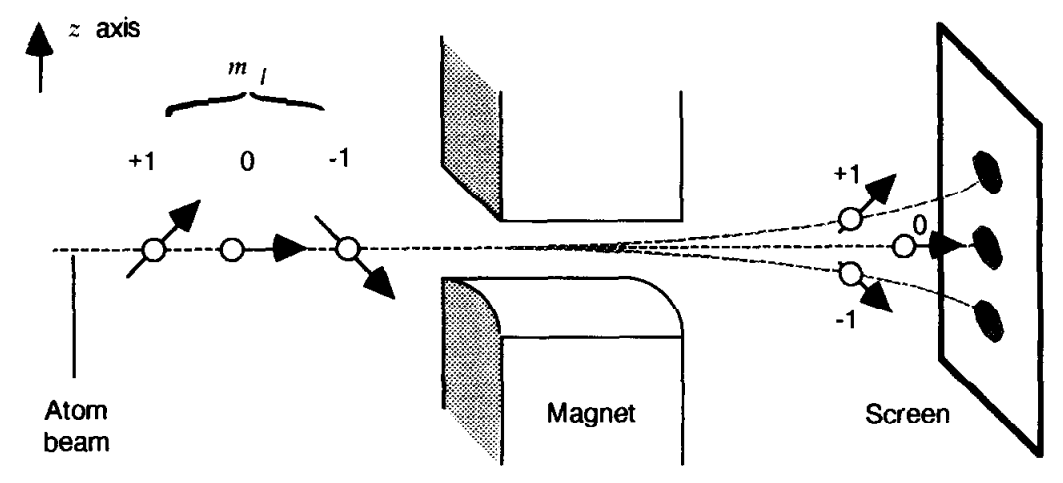
\includegraphics[scale=0.25]{figs/stern-gerlach.png}
    \caption{Schemat doświadczenia Sterna--Gerlacha}
    \label{fig:stern-gerlach}
\end{figure}

Wyniki doświadczenia można wyjaśnić na gruncie przedstawionej teorii. Rozważmy cząstkę neutralną
posiadającą niezerowy magnetyczny moment dipolowy \(\mu\) umieszczoną w niejednorodnym polu
magnetycznym. Założymy, iż pole magnetyczne jest dane wzorem

\begin{equation*}
\mathbf{B}=-\alpha x\mathbf{\hat{x}}+(\alpha z+B_0)\mathbf{\hat{z}}
\end{equation*}
gdzie osie \(z\) i \(y\) są zaznaczone na rysunku, natomiast \(\alpha\) jest wielkością małą w
porównaniu do \(B_0\). Zgodnie z równaniem Pauliego spinor \(\mathsf{\Psi}\) cząstki spełnia

\begin{equation*}
-\frac{\hbar^2}{2m}\Delta\mathsf{\Psi}-\mu\begin{bmatrix}
-\alpha x\Psi_-+(\alpha z+B_0)\Psi_+\\
-\alpha x\Psi_+-(\alpha z+B_0)\Psi_-
\end{bmatrix}=\im\hbar\pdv{\mathsf{\Psi}}{t}\,,
\end{equation*}
skąd otrzymujemy układ sprzężonych równań różniczkowych na składowe spinora

\begin{equation*}
\begin{split}
    & -\frac{\hbar^2}{2m}\Delta\Psi_+-\mu(\alpha z+B_0)\Psi_++\mu\alpha x\Psi_-=\im\hbar\pdv{\Psi_+}{t}\\
    & -\frac{\hbar^2}{2m}\Delta\Psi_-+\mu(\alpha z+B_0)\Psi_-+\mu\alpha x\Psi_+=\im\hbar\pdv{\Psi_-}{t}
\end{split}\,.
\end{equation*}
Podstawmy \(\Psi_+=\Psi_+'\e^{\im\omega_\text{L}t/2}\),
\(\Psi_-=\Psi_-'\e^{-\im\omega_\text{L}t/2}\), gdzie \(\omega_\text{L}\) jest częstością Larmora.
Otrzymujemy wówczas

\begin{equation*}
\begin{split}
    &-\frac{\hbar^2}{2m}\Delta\Psi_+'-\mu\alpha z\Psi_+'+\mu\alpha x\Psi_-'\e^{-\im\omega_\text{L}t}=\im\hbar\pdv{\Psi_+'}{t}\\
    &-\frac{\hbar^2}{2m}\Delta\Psi_-'+\mu\alpha z\Psi_-'+\mu\alpha x\Psi_+'\e^{+\im\omega_\text{L}t}=\im\hbar\pdv{\Psi_-'}{t}
\end{split}\,.
\end{equation*}
Dla uproszczenia pominiemy człon oscylacyjny, co prowadzi do rozprzężenia równań

\begin{equation*}
\begin{split}
    &-\frac{\hbar^2}{2m}\Delta\Psi_+'-\mu\alpha z\Psi_+'=\im\hbar\pdv{\Psi_+'}{t}\\
    &-\frac{\hbar^2}{2m}\Delta\Psi_-'+\mu\alpha z\Psi_-'=\im\hbar\pdv{\Psi_-'}{t}
\end{split}\quad.
\end{equation*}
Możemy zdefiniować wielkość

\begin{equation*}
\langle Q_\pm\rangle=\iiint_{\mathbb{R}^3}\Psi_\pm^*[\hat{Q}]\Psi_\pm\dd{^3\mathbf{r}}\,,
\end{equation*}
którą interpretujemy jako wartość oczekiwaną obserwabli \(Q\) dla cząstki w danym (a nie dowolnym)
stanie polaryzacyjnym. Z twierdzenia Ehrenfesta mamy więc

\begin{equation*}
\dv[2]{\langle z_\pm\rangle}{t}=\langle F_\pm\rangle\,,
\end{equation*}
gdzie \(\hat{F}_\pm=-\frac{1}{\hbar^2}\left[\hat{H}_\pm,[\hat{H}_\pm,z]\right]\), przy czym

\begin{equation*}
\hat{H}_\pm=-\frac{\hbar^2}{2m}\Delta\mp\mu\alpha z\,.
\end{equation*}
Otrzymujemy z powyższego

\begin{equation*}
\dv[2]{\langle z_\pm\rangle}{t}=\pm\frac{\mu\alpha}{m}\,,
\end{equation*}
czyli w przybliżeniu półklasycznym, w którym równanie ewolucji wartości oczekiwanych możemy
interpretować jako równanie przybliżonej trajektorii cząstek, widzimy, iż cząstki w różnych stanach
polaryzacyjnych odchylą się w przeciwne kierunki.

\subsection{Identyczne cząstki}

\subsubsection{Systemy dwucząstkowe}

Rozpatrujemy rozróżnialne cząstki bez spinu. Stan pojedynczej cząstki opisuje funkcja falowa
\(\Psi(\mathbf{r},t)\) ewoluująca zgodnie z równaniem Schr{\"o}dingera. Naturalnym uogólnieniem na
dwie cząstki jest opis układu za pomocą funkcji falowej \(\Psi(\mathbf{r}_1,\mathbf{r}_2,t)\), gdzie
\(\mathbf{r}_1\), \(\mathbf{r}_2\) są współrzędnymi związanymi z daną cząstką. Funkcja \(\Psi\)
spełnia równanie Schr{\"o}dingera postaci

\begin{equation*}
\boxed{\left[-\frac{\hbar^2}{2m_1}\Delta_1-\frac{\hbar^2}{2m_2}\Delta_2+V(\mathbf{r}_1,\mathbf{r}_2)\right]\Psi=\im\hbar\pdv{\Psi}{t}}\,,
\end{equation*}
gdzie \(\Delta_{1,2}=\pdv[2]{ }{x_{1,2}}+\pdv[2]{ }{y_{1,2}}+\pdv[2]{ }{z_{1,2}}\). Interpretacja
statystyczna brzmi teraz: \(\Psi^*\Psi\) jest gęstością prawdopodobieństwa znalezienia w ustalonej
chwili \(t\) cząstki 1 w położeniu \(\mathbf{r}_1\) \underline{i} cząstki 2 w położeniu
\(\mathbf{r}_2\). Warunek unormowania ma natomiast postać

\begin{equation*}
\int\Psi^*\Psi\dd{^3\mathbf{r}_1}\dd{^3\mathbf{r}_2}=1\,,
\end{equation*}
gdzie całkujemy dwukrotnie po całej przestrzeni \(\mathbb{R}^3\). Analogicznie obliczamy wartości
oczekiwane przez dwukrotne całkowanie po całej przestrzeni.\\

Można wyróżnić dwie istotne postaci funkcji potencjału.

\begin{itemize}

\item W przypadku \underline{nieoddziałujących} cząstek mamy
\(V=V_1(\mathbf{r}_1)+V_2(\mathbf{r}_2)\) i zakładając
\(\Psi=\Psi_1(\mathbf{r}_1,t)\Psi_2(\mathbf{r}_2,t)\) otrzymujemy dwa równania

\begin{equation*}
    \begin{split}
        &\left[-\frac{\hbar^2}{2m_1}\Delta_1+V_1\right]\Psi_1=\im\hbar\pdv{\Psi_1}{t}\\
        &\left[-\frac{\hbar^2}{2m_2}\Delta_2+V_2\right]\Psi_2=\im\hbar\pdv{\Psi_2}{t}
    \end{split}\quad.
\end{equation*}

\item W przypadku potencjału \underline{centralnego}
\(V(\mathbf{r}_1,\mathbf{r}_2)=V(|\mathbf{r}_1-\mathbf{r}_2|)\). W takim przypadku możemy skorzystać
ze znanej z klasycznego problemu Keplera metody separacji przez wprowadzenie nowych zmiennych
niezależnych \(\mathbf{r}=[x,y,z]\) i \(\mathbf{R}=[X,Y,Z]\)

\begin{equation*}
    \mathbf{r}:=\mathbf{r}_1-\mathbf{r}_2\,,\quad \mathbf{R}:=\frac{m_1\mathbf{r}_1+m_2\mathbf{r}_2}{m_1+m_2}\,.
\end{equation*}
Wówczas

\begin{equation*}
    \mathbf{r}_1=\mathbf{R}+\frac{m_2}{m_1+m_2}\mathbf{r}\,,\quad \mathbf{r}_2=\mathbf{R}-\frac{m_1}{m_1+m_2}\mathbf{r}\,,
\end{equation*}
skąd

\begin{equation*}
\begin{split}
    &\Delta_1=\pdv[2]{ }{\mathbf{r}}+\frac{m_1^2}{M^2}\pdv[2]{ }{\mathbf{R}}+\frac{2m_1}{M}\frac{\partial^2}{\partial \mathbf{r}\partial \mathbf{R}}\\
    &\Delta_2=\pdv[2]{ }{\mathbf{r}}+\frac{m_2^2}{M^2}\pdv[2]{ }{\mathbf{R}}-\frac{2m_2}{M}\frac{\partial^2}{\partial\mathbf{r}\partial \mathbf{R}}
\end{split}\quad,
\end{equation*}
gdzie \(M=m_1+m_2\). Po podstawieniu otrzymujemy

\begin{equation*}
    \left[-\frac{\hbar^2}{2M}\Delta_R-\frac{\hbar^2}{2m}\Delta_r+V(r)\right]\Psi=\im\hbar\pdv{\Psi}{t}\,,
\end{equation*}
gdzie \(m=m_1m_2/(m_1+m_2)\) to tzw. masa zredukowana, natomiast

\begin{equation*}
    \begin{split}
        &\Delta_R=\pdv[2]{ }{X}+\pdv[2]{ }{Y}+\pdv[2]{ }{Z}\\
        &\Delta_r=\pdv[2]{ }{x}+\pdv[2]{ }{y}+\pdv[2]{ }{z}
    \end{split}\quad.
\end{equation*}
Widzimy więc, iż \(\Psi=\Psi_R(\mathbf{R},t)\Psi_r(\mathbf{r},t)\), gdzie \(\Psi_R\) spełnia
równanie cząstki swobodnej o masie \(M\), natomiast \(\Psi_r\) spełnia równanie cząstki o masie
\(m\) w potencjale \(V(r)\). W świetle tych rozważań do równań opisujących atom wodoru należy
wprowadzić niewielką poprawkę przez zastąpienie we wszystkich wzorach masy elektronu masą
zredukowaną

\begin{equation*}
    m=\frac{m_\text{p}m_\text{e}}{m_\text{p}+m_\text{e}}=\frac{1836}{1837}m_\text{e}\approx 0.9995\,m_\text{e}\,.
\end{equation*}
\end{itemize}

\subsubsection{Bozony i fermiony}

Załóżmy, iż mamy układ dwóch cząstek o spinie 0 opisany funkcją falową
\(\Psi(\mathbf{r}_1,\mathbf{r}_2,t)\). Powyżej zakładaliśmy, iż cząstki te można odróżnić ze względu
na ich pewną wewnętrzną, fundamentalną cechę (np. proton i elektron). Zauważmy jednak, iż jeśli
cząstek tych fundamentalnie \underline{nie da się odróżnić} (mają jednakową masę, ładunek itp.) to
musi zachodzić 

\begin{equation*}
\boxed{\Psi(\mathbf{r}_1,\mathbf{r}_2,t)=\pm\Psi(\mathbf{r}_2,\mathbf{r}_1,t)}\,.
\end{equation*}
Istotnie gęstość prawdopodobieństwa \(|\Psi|^2\) znalezienia cząstki 1 w objętości
\(\dd{^3\mathbf{r}_1}\) i cząstki 2 w objętości \(\dd{^3\mathbf{r}_2}\) powinna być symetryczną
funkcją \(\mathbf{r}_1\) i \(\mathbf{r}_2\).

\begin{itemize}

\item Cząstki, dla których w powyższej równości zachodzi \(+\) nazywamy \underline{bozonami}.

\item Cząstki, dla których w powyższej równości zachodzi \(-\) nazywamy
\underline{fermionami}
\end{itemize}

Załóżmy teraz, iż cząstki te nie oddziałują ze sobą. Wówczas możemy rozwiązać równanie
Schr{\"o}dingera

\begin{equation*}
\left[-\frac{\hbar^2}{2m}\Delta_1-\frac{\hbar^2}{2m}\Delta_2+V(\mathbf{r}_1)+V(\mathbf{r}_2)\right]\Psi(\mathbf{r}_1,\mathbf{r}_2,t)=\im\hbar\pdv{\Psi}{t}
\end{equation*}
przez separację \(\Psi(\mathbf{r}_1,\mathbf{r}_2,t)=\alpha(\mathbf{r}_1,t)\beta(\mathbf{r}_2,t)\) co
pozwala określić funkcję \(\Psi\) jako iloczyn jednocząstkowych funkcji falowych dla cząstek w
odpowiednich potencjałach. Powyżej założyłem, iż cząstki są identyczne tj. \(m_1=m_2=m\) i potencjał
oddziaływania z zewnętrznym polem jest jednakowy (np. potencjał kulombowski dla jednakowych
ładunków). Taka funkcja nie spełnia jednak w ogólności \underline{wymogu symetryzacji}
\(\Psi(\mathbf{r}_1,\mathbf{r}_2)=\pm\Psi(\mathbf{r}_2,\mathbf{r}_1)\), możemy jednak skonstruować z
funkcji jednocząstkowych symetryczną lub antysymetryczną funkcję \(\Psi\) przez prostą superpozycję.
Wystarczy wziąć

\begin{equation*}
\Psi(\mathbf{r}_1,\mathbf{r}_2)=c_0\left\{\alpha(\mathbf{r}_1)\beta(\mathbf{r}_2)\pm\alpha(\mathbf{r}_2)\beta(\mathbf{r}_1)\right\}\,,
\end{equation*}
gdzie \(c_0\) jest pewną stałą normalizacyjną.

\subsubsection{Spin i zakaz Pauliego}

Powyższe rozważania dotyczą niestety jedynie bozonów o spinie 0. Istotnie w relatywistycznej
mechanice kwantowej daje się udowodnić tzw. \underline{twierdzenie o spinie i statystyce}
(\textit{spin--statistics theorem}), zgodnie z którym wszystkie cząstki o spinie całkowitym (0, 1,
2, ...) są bozonami, a wszystkie cząstki o spinie półcałkowitym (1/2, 3/2, 5/2, ...) są fermionami.
W świetle tego faktu powyższa konstrukcja funkcji falowej odnosi się jedynie do bozonów o spinie
0.\\

Pokażemy teraz jak zrobić to dla fermionów o spinie połówkowym (czyli elektronów). Ponownie
naturalnym uogólnieniem na system dwucząstkowy jest stwierdzenie, iż jego stan jest opisywany przez
pewien spinor \underline{czteroskładnikowy} \(\mathsf{\Psi}\) spełniający równanie Pauliego
(zakładamy potencjalność wszelkich sił zewnętrznych)

\begin{equation*}
\left[-\frac{\hbar^2}{2m}\Delta_1-\frac{\hbar^2}{2m}\Delta_2+V(\mathbf{r}_1)+V(\mathbf{r}_2)\right]\mathsf{\Psi}=\im\hbar\pdv{\mathsf{\Psi}}{t}\,.
\end{equation*}
Chcemy teraz utworzyć \(\mathsf{\Psi}(\mathbf{r}_1,\mathbf{r}_2,t)\) jako pewien ,,iloczyn''
dwuskładnikowych spinorów \(\mathsf{A}(\mathbf{r}_1,t)\), \(\mathsf{B}(\mathbf{r}_2,t)\)
spełniających jednocząstkowe równania

\begin{equation*}
\begin{split}
    &\left[-\frac{\hbar^2}{2m}\Delta_1+V(\mathbf{r}_1)\right]\mathsf{A}=\im\hbar\pdv{\mathsf{A}}{t}\\
    &\left[-\frac{\hbar^2}{2m}\Delta_2+V(\mathbf{r}_2)\right]\mathsf{B}=\im\hbar\pdv{\mathsf{B}}{t}
\end{split}\quad.
\end{equation*}
Można to zrobić wprowadzając \underline{iloczyn tensorowy} dwóch spinorów zdefiniowany jako

\begin{equation*}
\begin{bmatrix}
a_1\\a_2
\end{bmatrix}\otimes\begin{bmatrix}
b_1\\b_2
\end{bmatrix}=\begin{bmatrix}
a_1b_1\\
a_1b_2\\
a_2b_1\\
a_2b_2
\end{bmatrix}\quad.
\end{equation*}
Zauważmy, przy tym, iż działanie to nie jest przemienne. Co więcej, ponieważ dla sił potencjalnych
spinor \(\mathsf{A}\) można zapisać jako \(\alpha(\mathbf{r}_1,t)\mathsf{a}\), gdzie \(\alpha\) jest
funkcją, a \(\mathsf{a}\) jest stałym (w czasie i przestrzeni) spinorem. Wówczas jeśli
\(\mathsf{A}=\alpha\mathsf{a}\), \(\mathsf{B}=\beta\mathsf{b}\) spełniają równania jednocząstkowe,
to

\begin{equation*}
\mathsf{\Psi}(\mathbf{r}_1,\mathbf{r}_2,t)=\alpha(\mathbf{r}_1,t)\beta(\mathbf{r}_2,t)(\mathsf{a}\otimes\mathsf{b})
\end{equation*}
spełnia równanie dwucząstkowe. Teraz wymagamy antysymetryczności ze względu na podstawienia
\(\boxed{\mathbf{r}_1\leftrightarrow\mathbf{r}_2}\), \(\boxed{\mathsf{a}\leftrightarrow\mathsf{b}}\)
(tj. antysymetryczności ze względu na \underline{zamianę cząstek ze sobą}). Oczywiście powyższy
spinor nie spełnia w ogólności tego wymogu, ale możemy skonstruować z rozwiązań jednocząstkowych
antysymetryczny spinor poprzez superpozycję

\begin{equation*}
\mathsf{\Psi}(\mathbf{r}_1,\mathbf{r}_2)=c_0\bigg\{\alpha(\mathbf{r}_1)\beta(\mathbf{r}_2)(\mathsf{a}\otimes\mathsf{b})-\alpha(\mathbf{r}_2)\beta(\mathbf{r}_1)(\mathsf{b}\otimes\mathsf{a})\bigg\}\,,
\end{equation*}
gdzie pominęliśmy argument \(t\).\\

\textbf{Zakaz Pauliego}. Zauważmy, iż jeśli dwa elektrony są w jednakowym stanie spinowym
\(\mathsf{a}=\mathsf{b}\), to muszą być w różnych stanach położenia \(\alpha\neq\beta\) i odwrotnie
jeśli są w jednakowym stanie położenia, to muszą być w różnych stanach spinowych (inaczej nie
mielibyśmy w ogóle spinora dla całego układu). Ten warunek nazywamy \underline{zasadą wykluczenia
Pauliego}.

\subsubsection{Atom helu}

Neutralny atom o liczbie atomowej \(Z\) składa się z ciężkiego jądra o ładunku \(Ze\) otoczonego
\(Z\) elektronami. Najprostszym poza wodorem atomem jest hel (\(Z=2\)). Pomijając ruch jądra, możemy
założyć, że mamy do czynienia z układem dwucząstkowym, którego spinor spełnia równanie

\begin{equation*}
\begin{split}
&\Bigg[-\frac{\hbar^2}{2m}\Delta_1-\frac{\hbar^2}{2m}\Delta_2+\bigg(\frac{-2e^2}{4\pi\epsilon_0|\mathbf{r}_1|}+\\
&+\frac{-2e^2}{4\pi\epsilon_0|\mathbf{r}_2|}+\frac{e^2}{4\pi\epsilon_0|\mathbf{r}_1-\mathbf{r}_2|}\bigg)\Bigg]\mathsf{\Psi}(\mathbf{r}_1,\mathbf{r}_2,t)=\im\hbar\pdv{\mathsf{\Psi}}{t}\,.
\end{split}
\end{equation*}
Jeśli zignorujemy oddziaływanie elektron--elektron (które z pewnością nie jest małe, ale znacznie
upraszcza sytuację) to otrzymamy układ nieoddziałujących fermionów, dla którego możemy podać
rozwiązania separowalne. Istotnie możemy przedstawić \(\mathsf{\Psi}\) jako
\(\mathsf{\Psi}=\Psi\chi\), gdzie \(\Psi\) jest funkcją, skąd

\begin{equation*}
\Psi(\mathbf{r}_1,\mathbf{r}_2,t)=\Psi_{nlm}(\mathbf{r}_1,t)\Psi_{n'l'm'}(\mathbf{r}_2,t)\,,
\end{equation*}
gdzie \(\Psi_{nlm}\), \(\Psi_{n'l'm'}\) są stacjonarnymi rozwiązaniami jednocząstkowymi dla
elektronu w atomie wodoropodobnym danymi wzorami (\ref{eq:wodoropodobne}) przy zamianie
\(e^2\mapsto2e^2\). W szczególności istnieje stan podstawowy

\begin{equation*}
\Psi_1(\mathbf{r}_1,\mathbf{r}_2,t)=\Psi_{100}(\mathbf{r}_1,t)\Psi_{100}(\mathbf{r}_2,t)=c_0\e^{-\frac{r_1+r_2}{r_0}}\e^{-\frac{\im E_1't}{\hbar}}\,,
\end{equation*}
gdzie 

\begin{equation*}
E_1'=2E_1=-\frac{2\hbar^2}{2m(2r_0)^2}=-8\,\text{Ry}\approx  -109\,\text{eV}\,.
\end{equation*}
Zauważmy, iż \(\Psi_1\) jest symetryczne względem zamiany cząstek, więc w stanie podstawowym atomu
helu elektrony muszą być w różnych stanach spinowych. Energia stanu podstawowego helu określona
eksperymentalnie wynosi ok. \(-79\,\text{eV}\). Niezgodność wynika oczywiście z faktu pominięcia
oddziaływania elektron--elektron.\\

\textbf{Nomenklatura stanów atomowych}. Stan atomu wodoropodobnego (jeden elektron przyciągany przez
nieruchome jądro o ładunku \(Ze\)) jest opisany funkcją falową (\ref{eq:wodoropodobne}). Z powodów
historycznych stany numerowane liczbami kwantowymi \(n\) (główną), \(l\) (poboczną), \(m\)
(magnetyczną) są oznaczane również w następujący sposób:

\begin{itemize}

\item zapisujemy główną liczbę kwantową \(n\)

\item następnie piszemy literę \(s\), \(p\), \(d\), \(f\), \(j\), \(k\), \(l\) i dalej alfabetycznie
dla kolejnych pobocznych liczb kwantowych \(l=0,1,...,n-1\)

\item magnetycznej liczby kwantowej nie zapisujemy

\end{itemize}
Ponieważ dla atomów wieloelektronowych przy pominięciu oddziaływań elektron--elektron rozwiązaniami
są odpowiednie kombinacje funkcji falowych atomu wodoropodobnego więc korzystamy z analogicznej
nomenklatury dopisując dodatkowo w wykładniku liczbę elektronów w danym stanie (ze względu na zakaz
Pauliego nie mogą być one wszystkie np. w stanie podstawowym dla \(Z\geq 3\)). Tak więc np. zapis

\begin{equation*}
(1s)^2(2s)^2(2p)^2
\end{equation*}
określa konfigurację: 2 elektrony w stanie podstawowym; 4 elektrony w pierwszym stanie wzbudzonym,
po dwa dla liczb pobocznych 0, 1.

\subsubsection{Struktura pasmowa}

Przeanalizujemy teraz niezwykle uproszczony model jednowymiarowej sieci krystalicznej. W tym celu
poszukamy rozwiązań jednowymiarowego niezależnego od czasu równania Schr{\"o}dingera

\begin{equation*}
\left[-\frac{\hbar^2}{2m}\dv[2]{}{x}+V(x)\right]\psi=E\psi\,,
\end{equation*}
dla potencjału przestrzennie okresowego z okresem \(a\) tj. \(V(x+a)=V(x)\) dla każdego
\(x\in\mathbb{R}\).\\

\textbf{Twierdzenie Blocha}. Niezwykle pomocnym twierdzeniem przy rozwiązywaniu powyższego problemu
jest twierdzenie Blocha, które mówi, iż funkcja \(\psi\) spełniająca

\begin{equation*}
\boxed{\psi(x+a)=\e^{\im qa}\psi(x)}\,,
\end{equation*}
gdzie \(q\) jest pewnym parametrem rzeczywistym spełnia niezależne od czasu równanie
Schr{\"o}dingera dla okresowego potencjału z okresem \(a\).\\

Założymy, że potencjał składa się z ciągu pików funkcji delta Diraca (tzw. grzebień Diraca)

\begin{equation*}
V(x)=\alpha\sum_{i=0}^{\infty}\delta(x-ia)\,.
\end{equation*}
Jest to uproszczony \underline{model Kroniga--Penneya}. Rozważmy obszar \(x\in(0;a)\). W tym
obszarze funkcja falowa spełnia równanie cząstki swobodnej, więc

\begin{equation*}
\psi(x)=a\sin (kx)+b\cos(kx)\,,
\end{equation*}
gdzie \(k=\sqrt{2mE}/\hbar\). Zgodnie z twierdzeniem Blocha dla \(x\in(-a;0)\) funkcja falowa ma
postać

\begin{equation*}
\psi(x)=\e^{-\im qa}(a\sin (kx)+b\cos(kx))\,.
\end{equation*}
Z ciągłość \(\psi\) i wartości pochodnej w 0 otrzymujemy warunek

\begin{equation*}
\cos(qa)=\cos(ka)+\frac{m\alpha}{\hbar^2k}\sin(ka)\,.
\end{equation*}
Warunek ten wyznacza dozwolone energie cząstki w okresowym potencjale. Pozostaje nałożyć pewien
warunek na \(q\). Zrobimy to, nakładając periodyczny warunek brzegowy

\begin{equation*}
\psi(x+Na)=\psi(x)\,,
\end{equation*}
gdzie \(N\) jest bardzo dużą liczbą naturalną rzędu liczby Avogadro (\(\sim10^{23}\)). Z powyższego
i twierdzenia Blocha mamy więc

\begin{equation*}
q = \frac{2\pi n}{Na}\,,\quad n\in\mathbb{Z}\,.
\end{equation*}
Numeryczne wyznaczenie dozwolonych energii pokazuje, iż tworzą one pasma dozwolonych energii, w
obrębie których zasadniczo każda energia jest dopuszczalna (dla bardzo dużych \(N\)).

\begin{figure}[ht]
    \centering
    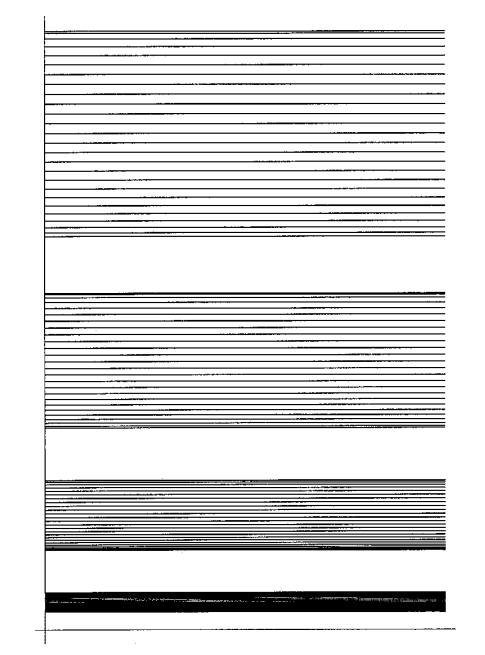
\includegraphics[scale=0.5]{figs/bands.png}
    \caption{Struktura pasmowa dla przestrzennie okresowego potencjału. Wewnątrz pasm zasadniczo każda energia jest dozwolona dla dużych \(N\).}
    \label{fig:bands}
\end{figure}

\end{document}